
\documentclass[12pt,spanish]{report}

%include spanish accents and tilde
\usepackage[T1]{fontenc}
\usepackage[utf8]{inputenc}

% ------------------- Colors --------------------------------------------------------------------------- %
%color package
%\usepackage{xcolor}
\usepackage[table]{xcolor}
% ==== hyper references colors ==== %
\definecolor{myLinkColor}{rgb}{0.6, 0.4, 0.1}
\definecolor{myUrlColor}{rgb}{0.1, 0.1, 0.7}

% ==== document control colors ==== %
% Each color specifies what is to be done with the text coloured with it
% command: \textcolor{color}{text paragraph}
\definecolor{commentary}{rgb}{0.5, 0.5, 0.5} %invisible mode: \iffalse ... \fi
\definecolor{FIXME}{rgb}{0.9, 0.1, 0.1} %changes have to be made here
\definecolor{TODO}{rgb}{0.2, 0.8, 0.4} %replace this with something else. probably an image

% ==== OpenOffice Draw colors ====
\definecolor{OODlightblue}{RGB}{207, 231, 245}
\definecolor{OODskyblue10}{RGB}{153, 204, 255}
\definecolor{OODskyblue09}{RGB}{102, 153, 204}
\definecolor{OODskyblue08}{RGB}{51, 102, 153}

%Aplicar un color a un bloque de texto: \textcolor{FIXME}{ALGO}

% ==== other colors ==== %
\definecolor{colorUNQ}{RGB}{132, 0, 16}

% ------------------- margins control ------------------------------------------------------------------ %
%document margins control package
\usepackage{geometry}
%https://en.wikibooks.org/wiki/LaTeX/Page_Layout
\textheight = 620pt %Change the space occupied by the text. Default = 592pt, so text will occupy more space now
\textwidth  = 450pt %Change the space occupied by the text. Default = 390pt, so text will occupy more space now
\marginparwidth = 1pt % Default 35pt
\hoffset = 1pt

% ------------------- Footers and headers -------------------------------------------------------------- %
%total number of pages package 
\usepackage{lastpage} %\pageref{LastPage} to get the last page (* to remove reference)

%headers and footers package
\usepackage{fancyhdr} %\thispagestyle{fancy} to revert 'plain' page style from \chapter to fancy
\fancypagestyle{fancy_normalPage}
{
    \fancyhf{} % clear all header and footer fields
    %\fancyhead[L]{\rightmark}%\chaptername\ \thechapter}
    \fancyhead[R]{Página \thepage\ de \pageref*{LastPage}} %the * removes the reference
    \renewcommand\headrule %change header properties
    {
      \color{colorUNQ}
      \vspace{5pt}
      \hrule height 0.1mm width\headwidth
    }
    \renewcommand{\footrulewidth}{0mm} %erase footer line
}
% ------------------- Chapter related ------------------------------------------------------------------ %
%\renewcommand{\chaptername}{Capítulo} %Rename chapter name 
\usepackage{titlesec} %chapter names
\titleformat{\chapter}[display]
  {\normalfont\bfseries\centering}{}{0cm}{\Huge} %Delete the "Chapter n" header for each chapter
  \titlespacing*{\chapter}{0cm}{-2cm}{1cm} %resize title space {right}{above}{below}

% ------------------- Images --------------------------------------------------------------------------- %
%images package
\usepackage{graphicx}
%\graphicspath{ {resources/} }
\renewcommand{\figurename}{Figura} %name of the Figures

\iffalse %HOW TO USE FIGURES:
    \begin{figure}[!ht]
      \centering
        \includegraphics[width=\textwidth]{figname.png}
        \caption{description} %Caption appears below the image. place this line before \includegraphics to make it appear above it
        \label{fig:\thefigure}  %or \label{fig:aNumber}
    \end{figure}
    
    %referencing a figure
    \ref{fig:number} %if \thefigure is 1.1, then number = 1.1. if you used aNumber, number = aNumber
    \autoref{fig:number} %for the complete name hyperref (Figure: \thefigure)
\fi

% ------------------- Math package --------------------------------------------------------------------- %

\usepackage{amsmath}

\iffalse %EQUATIONS EXAMPLES
    %Normal equation
    \begin{equation}\label{eq:\theequation} %or \label{eq:aNumber} 
    \mbox{\Large\( % Change size of the containing box. Normal size: \normalsize
    \begin{split} %Align equations with & and separate with \\
        y_1 & = \sum_{i=0}^{\infty} a_i x^i \\ %\notag para sacar el label
        y_2 & = \sum_{i=\sigma}^{\Phi} a_i x^i
    \end{split}
    \)} %
    \end{equation}
    
    %referencing an equation
    \eqref{eq:number} %equation hyperref with parenthesis. available with \usepackage{hyperref}
    \ref{eq:number} %reference to the equation, without parenthesis
    \autoref{eq:number} %for the complete name hyperref (Equation:\theequation)
    
    %Aligned equation (with &)
    \begin{align}\label{eq:2}
        e^{i\pi} & = \cos(\pi) + i\sin(\pi) \notag \\  %To remove tag and move to the next line (\\)
            & = -1 .
    \end{align}
    
    %Piecewise equation
    \[
     fe(t) =
      \begin{cases} 
    
           1    &  0 \leq t \leq 5
           0    & e.o.c. \notag \\
      \end{cases}
    \]
    
    %Equations formatting: https://en.wikipedia.org/wiki/Help:Displaying_a_formula
    %Online equations editor: https://www.codecogs.com/latex/eqneditor.php
\fi

% ------------------- Tables example ------------------------------------------------------------------- %
\iffalse %This section does not include a user package. It's just an example
%https://en.wikibooks.org/wiki/LaTeX/Tables
\begin{table}[!ht]
  \begin{center}
    \begin{tabular}{| l c r |}
    \hline
    1 & 2 & 3 \\
    4 & 5 & 6 \\
    7 & 8 & 9 \\
    \hline
    \end{tabular}
  \end{center}
  \caption{A simple table}
\end{table}
\fi

\renewcommand{\tablename}{Tabla} %name of the Tables

% ------------------- Hyperreferences ------------------------------------------------------------------ %
%Hyperref packages
\usepackage{hyperref}
\hypersetup{
    colorlinks,
    citecolor=green,
    filecolor=black,
    linkcolor=colorUNQ,
    urlcolor=colorUNQ
}
%\urlstyle{same}

% ------------------- adding code/scripts -------------------------------------------------------------- %

\usepackage{listings}

\definecolor{matlabComment}{RGB}{34, 139, 34} 
\definecolor{matlabString}{RGB}{160, 32, 240} 
\definecolor{matlabNumber}{RGB}{255, 128, 102} 
\definecolor{matlabKeyword}{RGB}{0, 0, 255} 

\definecolor{cComment}{RGB}{0, 128, 0} 
\definecolor{cString}{RGB}{160, 32, 240} 
\definecolor{cNumber}{RGB}{255, 128, 0} 
\definecolor{cKeyword}{RGB}{128, 0, 255} 
\definecolor{backgroundColour}{RGB}{227,231,245}

\lstdefinestyle{CStyle}{
	backgroundcolor=\color{backgroundColour},   
	commentstyle=\color{cComment},
	keywordstyle=\color{cKeyword},
	numberstyle=\tiny\color{cNumber},
	stringstyle=\color{cString},
	basicstyle=\footnotesize,
	breakatwhitespace=false,         
	breaklines=true,                 
	captionpos=b,                    
	keepspaces=true,                 
	numbers=left,                    
	numbersep=5pt,                  
	showspaces=false,                
	showstringspaces=false,
	showtabs=false,                  
	tabsize=2,
	language=C
}

% to inclode block of code: \lstinputlisting[language=language]{resources/sourceName.languageType}
% to encapsulate code: \begin{lstlisting}[frame=single] code... \end{lstlisting}

% ------------------- subscripts and superscripts fix -------------------------------------------------- %
%\usepackage{fixltx2e}
%subscript: x\textsubscript{y} or \(x_y\)
%superscript: x\textsuperscrip{y} or \(x_y\)
%Fix in headings: \texorpdfstring (from \usepackage{hyperref})

% ------------------- Apply stylization ---------------------------------------------------------------- %
%Remove paragraph indentation
\setlength{\parindent}{0pt}
\pagestyle{fancy_normalPage} %set pagestyle to my pagestyle (fancy_normalPage)
%Stylize new paragraphs. To use it explicitely: " \par " 
\setlength{\parindent}{0.3cm} % Paragraph indentation 
\setlength{\parskip}{0.3cm} % Space between paragraphs

% ------------------- Table of contents ---------------------------------------------------------------- %
\renewcommand{\contentsname}{Índice de contenidos}

\renewcommand{\listfigurename}{Índice de figuras}

% ------------------- Contadores de subsecciones ---------------------------------------------------------------- %
\setcounter{secnumdepth}{4} % seting level of numbering (default for "report" is 3). With ''-1'' you have non number also for chapters
\setcounter{tocdepth}{4} % if you want all the levels in your table of contents


% ------------------- Document ------------------------------------------------------------------------- %


\begin{document}

\begin{titlepage}
%https://en.wikibooks.org/wiki/LaTeX/Title_Creation

\includegraphics[width=\textwidth]{resources/0-UNQlogo.jpg}\\ %University logo

\begin{center}
	\text{\large Departamento de Ciencia y Tecnología}\\[0.2cm] % 
	\text{\large Ingeniería en Automatización y Control Industrial}\\[0.5cm] 
	\textsc{\LARGE \textcolor{colorUNQ}{Control automático del equipo Updown} }\\[1cm] 
	\textbf{\large Olivieri, Ian Paulo}\\ [1cm]
\end{center}	

\textbf{\normalsize Director:}\\
\text{\normalsize \hspace{3cm} Pernia, Eric Nicolás}\\

\textbf{\normalsize Co-director:}\\
	\text{\normalsize \hspace{3cm} x}\\

\textbf{\normalsize Jurado:}\\
	\text{\normalsize \hspace{3cm} Safar, Felix }\\
	\text{\normalsize \hspace{3cm} Juarez, José}\\
	\text{\normalsize \hspace{3cm} y}\\
	\text{\normalsize \hspace{3cm} z}\\[1cm]

	%\rule{\linewidth}{0.1mm} %Separation line
\begin{flushright}
	\text{\normalsize Presentación: Septiembre de 2017}\\
	\text{\normalsize Quilmes, Buenos Aires, Argentina.}\\ [0.5cm]
\end{flushright} 

\end{titlepage}

\thispagestyle{empty}
\begin{center}

	\textbf{\huge Resumen }\\[1cm] 

\end{center}



Resumen del proyecto (1 carilla)


% ==== Tabla de contenidos ==== %
\tableofcontents

% ==== índice de figuras ==== %
\listoffigures

% ==== índice de figuras ==== %
\listoftables


\chapter{Introducción}
\thispagestyle{empty}


\section{Marco temático} \label{sec:\thesection}
\subsection{Esculturas cinéticas}
\subsubsection{Definición}
Las esculturas cinéticas (kinetic sculpture en inglés) son estructuras tridimensionales en donde el movimiento es una parte fundamental del conjunto. Para lograr el efecto de movimiento en el espacio estos sistemas se construyen con partes móviles que pueden cambiar de posición ya sea naturalmente por acción del viento, como se ve en la figura \ref{fig:1.1}, o de manera forzada.
% https://www.youtube.com/watch?v=D2HF-1xjpP8

\begin{figure}[!ht]
	\centering
	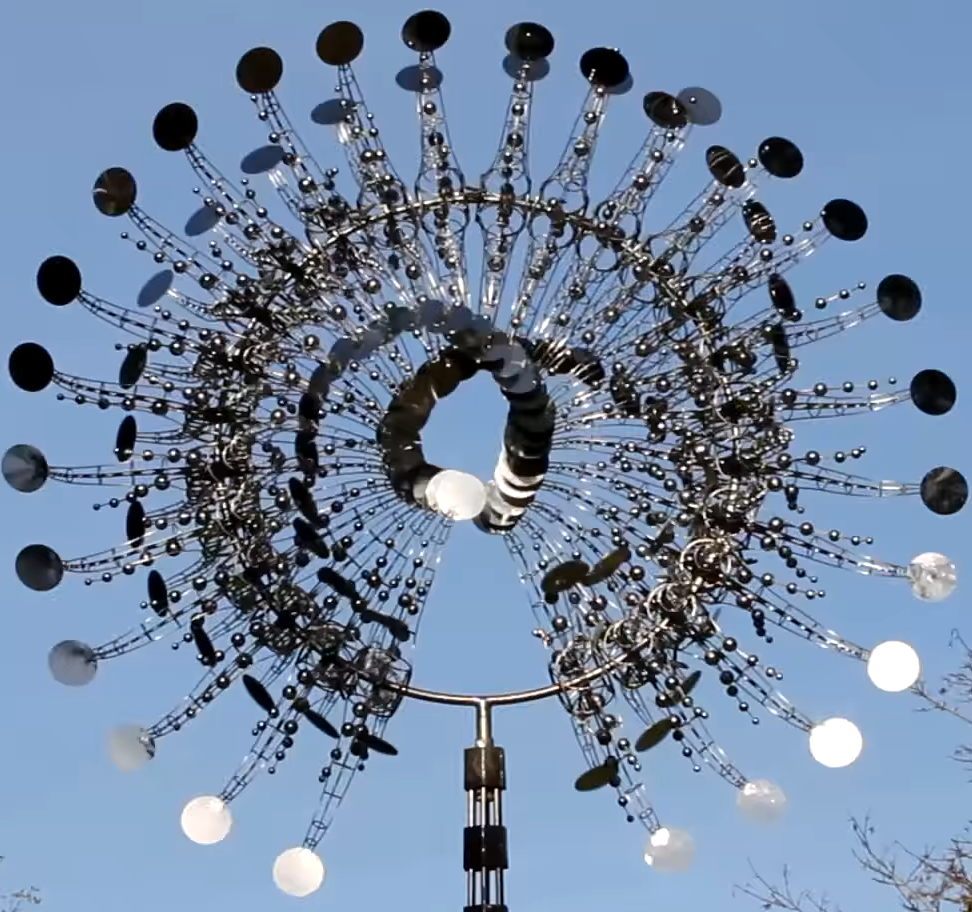
\includegraphics[width=10cm,scale=1]{resources/1_1-kinSculp.png}
	\caption{ Ejemplo de escultura cinética movida por aire, por Anthony Howe. Fuente:  \href{https://www.youtube.com/watch?v=N-1LpikCSR4}{LINK al video} }
	\label{fig:\thefigure}
\end{figure}

\newpage
\subsubsection{Aplicaciones y estado actual del arte}
Al ser obras que caen dentro del campo artístico suelen presentarse en museos y utilizarse para fines decorativos ya sea en parques o eventos. Sin embargo, el nivel de ingeniería y diseño que algunas de ellas requieren las tornan un interesante desafío intelectual y creativo.

Las aplicaciones puntuales de estructuras cinéticas a las que se hará foco en este informe, debido a la naturaleza del proyecto final, son aquellas en donde el efecto espacial se logra a través del movimiento en el eje vertical de objetos esféricos mediante motores. 

Un ejemplo de aplicación de estas características se puede ver en la figura \ref{fig:1.2}. Allí se muestra una escultura presentada en el Museo de BMW, en Munich, Alemania, en donde 714 esféras metálicas son coordinadas para formas figuras como olas, gotas, y hasta la silueta de un auto.

\begin{figure}[!ht]
	\centering
	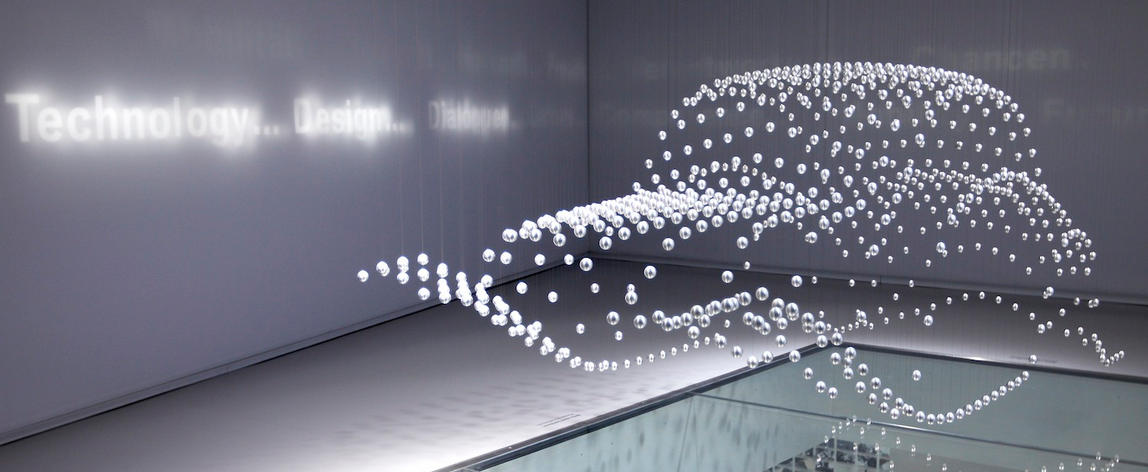
\includegraphics[width=15cm,scale=1]{resources/1_2-kinSculp.png}
	\caption{ Escultura cinética en el museo BMW. Fuente: \href{https://www.youtube.com/watch?v=HVhVClFMg6Y}{LINK al video} }
	\label{fig:\thefigure}
\end{figure}

Otro ejemplo de aplicación se puede ver en la figura \ref{fig:1.3}, en una obra presentada por la empresa Build Up en un centro comercial en Fukuoka, Japón. Allí se instalaron 1000 luminarias esféricas RGB dispuestas en una matriz de 25x40 para generar figuras tridimensionales como planos y gausseanas, entre otras. En este caso los efectos espaciales se logran coordinando el movimiento de cada esfera independientemente, cada una manejada por un equipo motorizado.
\begin{figure}[!ht]
	\centering
	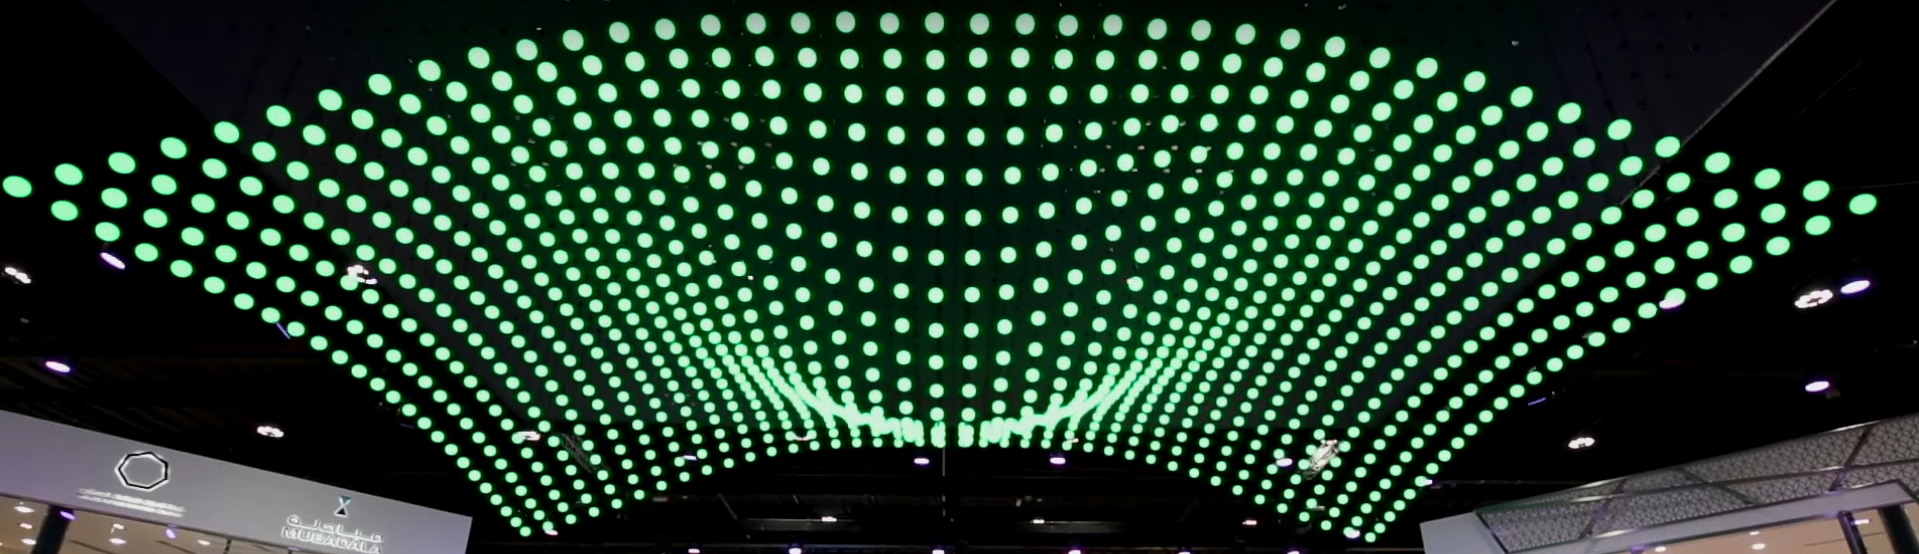
\includegraphics[width=15cm,scale=1]{resources/1_3-kinSculp.png}
	\caption{ Escultura cinética por parte de Build Up. Fuente: \href{https://www.youtube.com/watch?v=ICixCazf6-k}{LINK al video} }
	\label{fig:\thefigure}
\end{figure}

%\newpage


\subsection{Sistemas de iluminación} 
\subsubsection{Equipos de luces}
En cualquier espectáculo o evento la iluminación es una parte vital del show, y a medida que estos fueron evolucionando también lo hicieron los equipos de luces. Partiendo de aparatos fijos en donde solo se podía variar la intensidad de luz, se pueden conseguir hoy en día dispositivos complejos con decenas de parámetros controlables.\\
Un notable ejemplo es el \href{http://preworks.at/index.php/en/products/led-automated-luminairies/shapeshifter}{Shapeshifter}, figura \ref{fig:1.4}, que cuenta con 7 módulos leds que pueden ser manejados independientemente.

\begin{figure}[!ht]
	\centering
	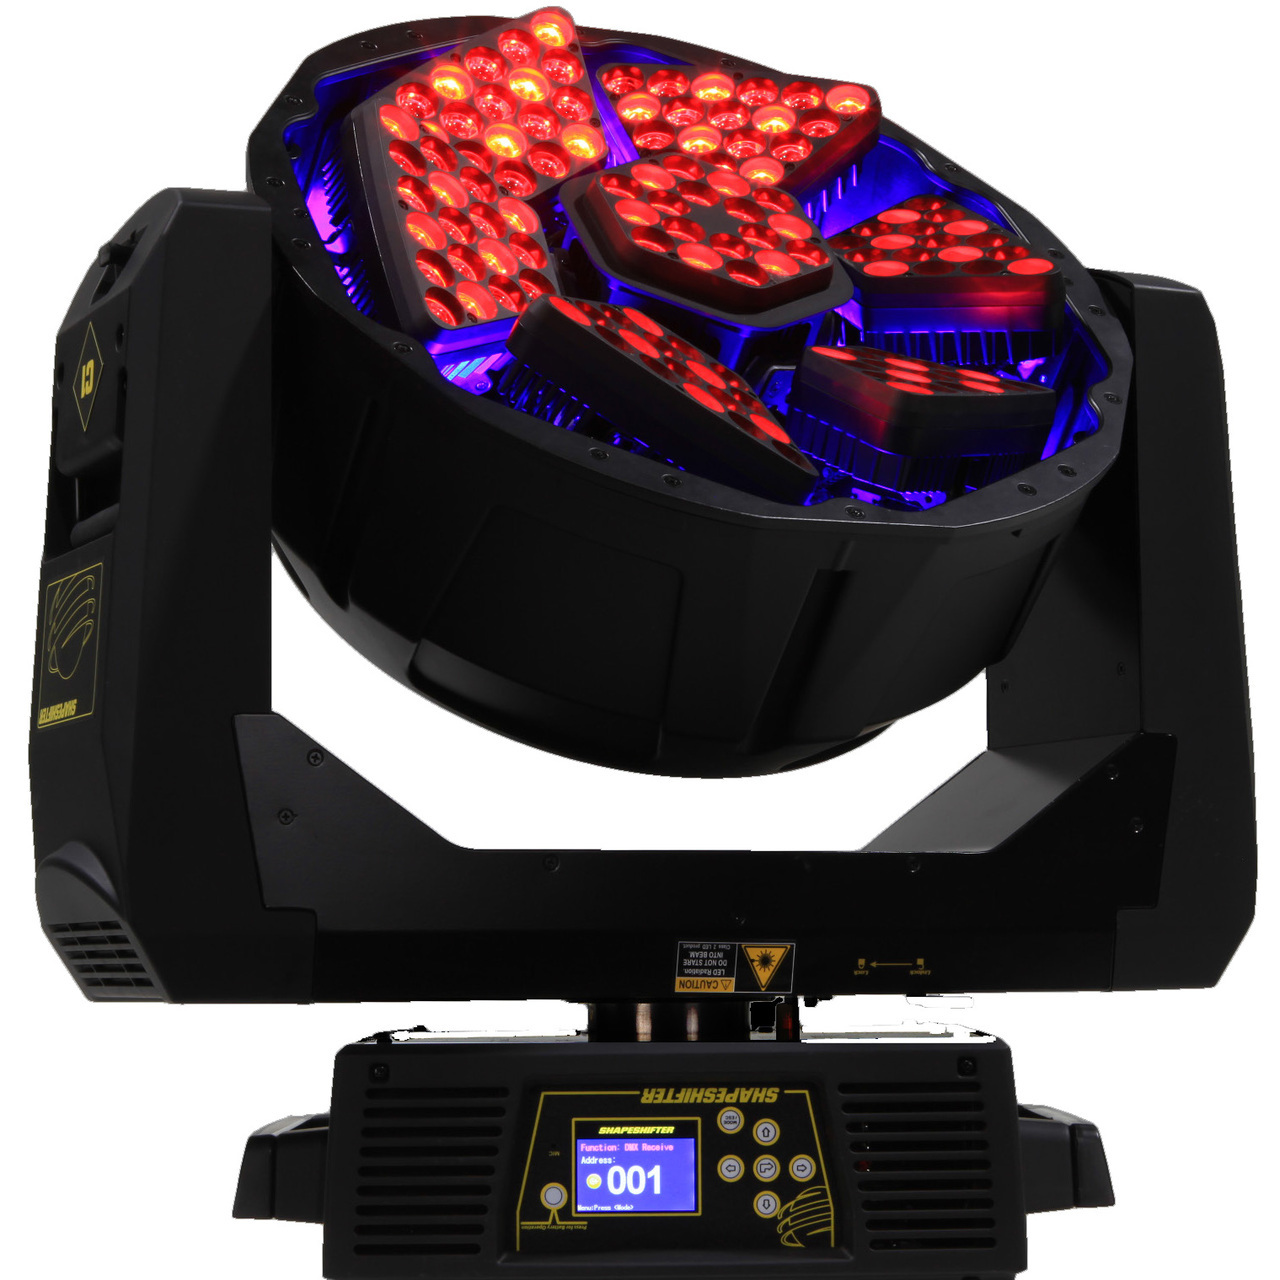
\includegraphics[width=7cm,scale=1]{resources/1_4-shapeshifter.jpg}
	\caption{Shapeshifter, de High End Systems. Fuente: \href{https://www.youtube.com/watch?v=LIIE3zZscYY}{LINK al video} }
	\label{fig:\thefigure}
\end{figure}

En el caso del sistema visto en la figura \ref{fig:1.3}, los parámetros controlables de los equipos son la posición, velocidad y colores de cada esfera.

\subsubsection{Consolas de control de luminaria}
Para controlar los sistemas de luces es necesario utilizar unas consolas especiales. Estas se comunican con las luminarias utilizando el estándar \textbf{DMX} y le indican a cada equipo el valor de sus parámetros en todo momento.

La manera más común para generar un efectos es indicando la progresión de uno o más parámetros desde un tiempo inicial a uno final. Al cambio de los parámetros entre 2 instantes de tiempo se las llama \textit{cues}, o entradas, y cuyo conjunto forma los efectos. \\
Dentro de las consolas que hay en el mercado para este tipo de control de equipos se pueden destacar las \href{https://www.highend.com/products/consoles}{consolas hog 4} de High End Systems, como la que se muestra en la figura \ref{fig:1.5}.

Otra manera generarlos es a partir de equipos y softwares, como el \href{https://www.madrix.com/}{Madrix}, que tienen la capacidad de convertir videos a variaciones de parámetros, lo cual lo hace especialmente útil cuando se quieren crear \href{https://www.youtube.com/watch?v=mdbl5ks7Nu0}{efectos lumínicos complejos}.


\begin{figure}[!ht]
	\centering
	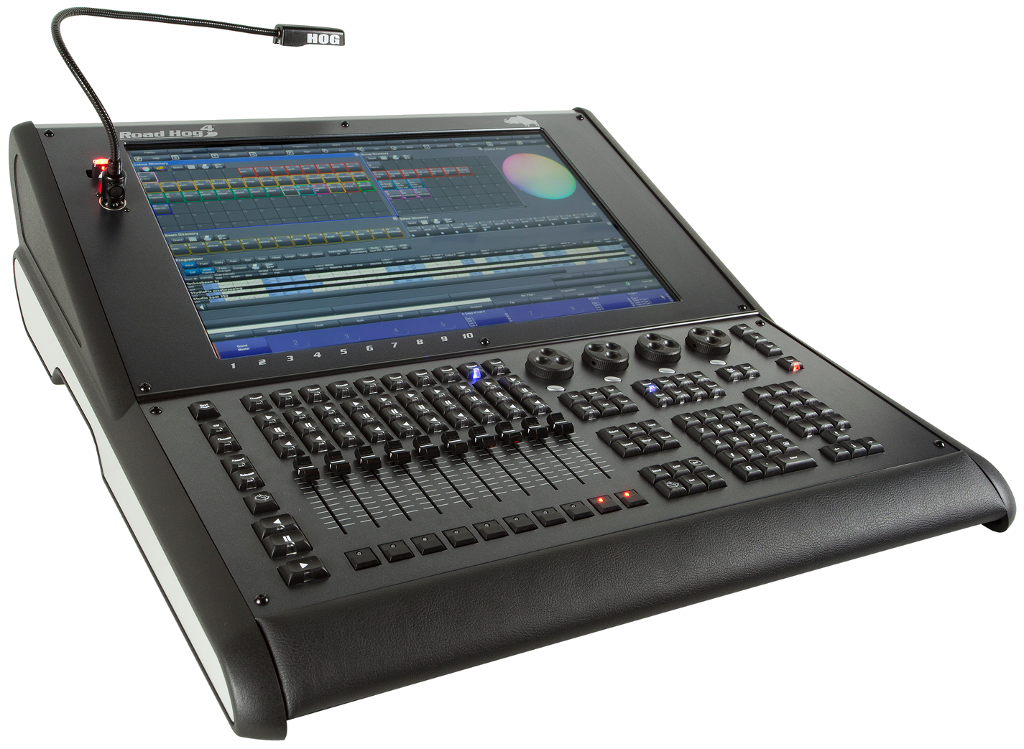
\includegraphics[width=10cm,scale=1]{resources/1_5-consolaHOG.png}
	\caption{Consola Hog4, de High End Systems. Fuente: \href{https://www.highend.com/products/consoles}{LINK a la imágen}}
	\label{fig:\thefigure}
\end{figure}

\newpage
\section{DMX} \label{sec:\thesection}
\subsection{Definición e historia}
DMX, de \textit{Digital MultipleX}, es un estándar de comunicación digital ámpliamente utilizado para el control de sistemas de iluminación. 

El estándar DMX512, donde 512 significa que se envían 512 piezas de información, fue creado por la \textit{United States Institute for Theatre Technology} (USITT) en 1986 y transformado en DMX512/1990 tras una revisión de la USITT. En 1998 la \textit{Entertainment Services and Technology Association} (ESTA) cuadró DMX dentro de los estándares ANSI, modificación que fue aprovada por el instituto (ANSI) en 2004. Finalmente, en 2008 DMX tuvo una nueva revisión y se llegó a la versión actual llamada "E1.11 – 2008, USITT DMX512-A", o simplemente DMX512-A. A pesar de esto, el nombre comúnmente conocido del estándar es simplemente DMX, aunque no es indistinto ya que hay diferencia de compatibilidad entre las diferentes versiones.


\subsection{Capa física}
\subsubsection{Cableado y conectores}
DMX empléa el estándar EIA-485 como capa física, por lo que emplea por lo menos 3 lineas; A, B y C, en donde A y B es por los datos son transmidos, y C es masa. Los conectores utilizados son los XLR, tanto de 5 como de 3 pines. Un ejemplo del cable se puede ver en la figura \ref{fig:1.6} \\

\begin{figure}[!ht]
	\centering
	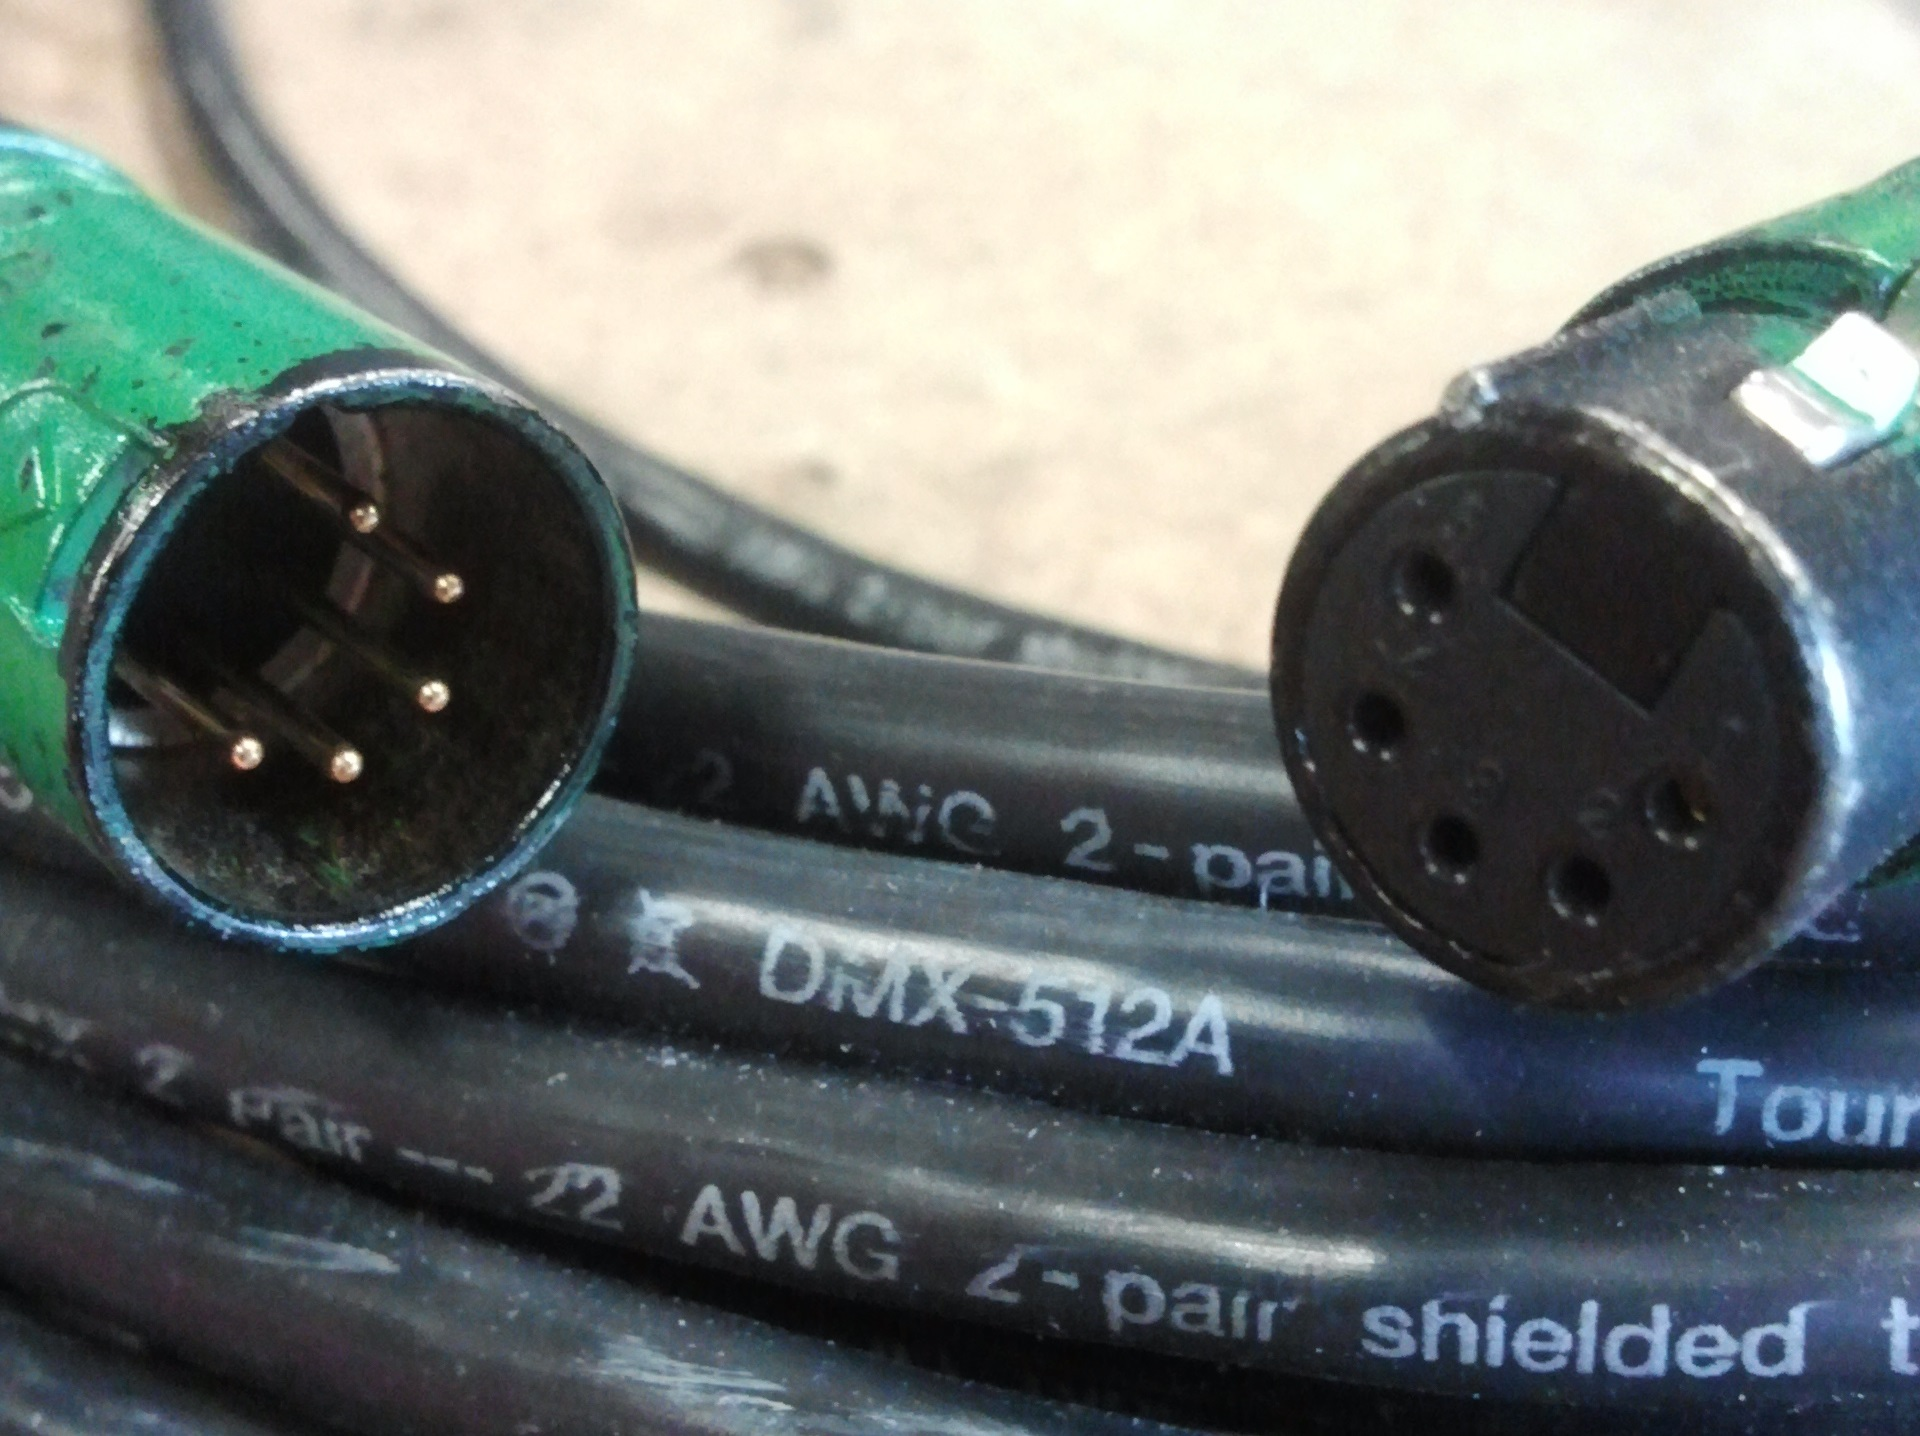
\includegraphics[width=8cm,scale=1]{resources/1_6-cableDMX.jpg}
	\caption{Cable DMX con conector XLR5. Fuente: wikipedia}
	\label{fig:\thefigure}
\end{figure}

\subsubsection{Topología}
La red de DMX consiste en un maestro y varios esclavos, conectados con una topología de bus multidrop (MDB) con nodos conectados entre sí, lo que normalmente se denomina como topología \textit{daisy chain}. En otras palabras, todos los equipos a controlar tienen una entrada y una salida conectadas entre sí, de manera tal de que se puede conectar un equipo y apartir de este equipo conectar el siguiente, y así sucesivente, como se ve en la figura \ref{fig:1.7}. Esto permite que el conexionado sea simple y que la red pueda ser fácilmente extendida.

\begin{figure}[!ht]
	\centering
	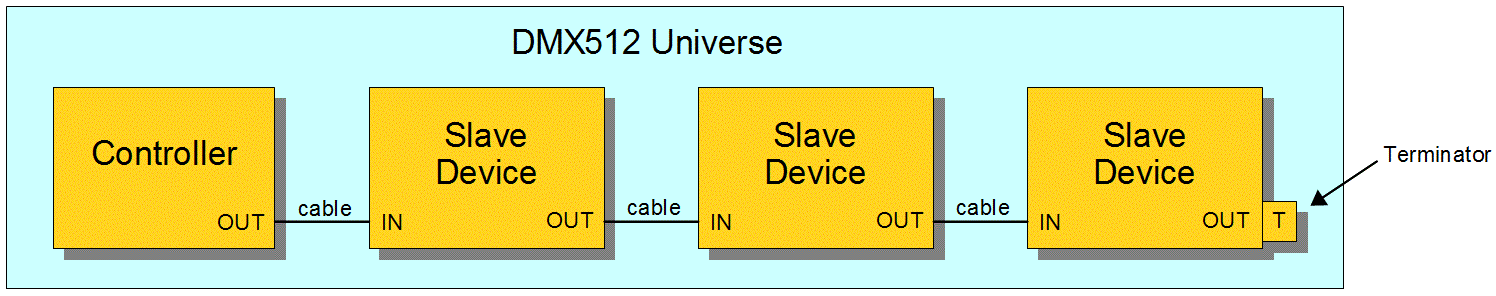
\includegraphics[width=15cm,scale=1]{resources/1_7-topologiaDMX.png}
	\caption{Conexionado en una red DMX. Fuente: wikipedia}
	\label{fig:\thefigure}
\end{figure}

\subsubsection{Señal}
La señal de DMX es de tipo diferencial, como es indicado en EIA-485, de 5 Volts de pico, y los datos se envían asincrónicamente de manera serie con una tasa de transmisión de 250Kbits por segundo que equivale a una duración de bit de 4\(\mu \)s.


\subsection{Capa de enlace de datos}
\subsubsection{Subcapa de control de enlace lógico}
La trama DMX, visible en la figura \ref{fig:1.8} consta de las siguientes partes:
%Fuentes: Fhttp://www.dmx512-online.com/packt.html 

\begin{itemize}
	\item \textbf{Idle} y \textbf{MTBP} (Mark Time Between Packets): estado de HIGH en la linea que indica la ausencia de señal de DMX. En caso de que se supere el tiempo máximo de 1 segundo sin datos, se considera que hubo una pérdida en la conexión.
	\item \textbf{Break}: estado de LOW en la línea utilizado para separar las tramas entre sí.
	\item \textbf{MAB} (Mark After Break): estado en HIGH enviado luego de un Break. Este estado suele traer problemas de compatibilidad ya que fue cambiado de una duración de 4\(\mu \)s a 8\(\mu \)s en la versión de DMX512 de 1990.
	\item \textbf{Slots}: son datos con formato 8N2 (un bit de start (LOW), 8 bits de datos, 2 bits de stop (HIGH) y sin paridad), y pueden ser:
	\begin{itemize}
		\item \textbf{SC} (Start Code): es el Slot 0, enviado luego de un MAB, para indicar el principio del payload. Todos los bits de datos equivalen a LOW en este estado.
		\item \textbf{Channels}: contienen la información que quiere ser enviada a los equipos de DMX. El conjunto de los 8 bits de datos pueden tomar un valor de 0 a 255. En total pueden haber un máximo de 512 canales enviados.
	\end{itemize}
	\item \textbf{MTBF} (Mark Time Between Frames): estado opcional de HIGH en la linea que puede agregarse antes del bit de start de cada canal.
\end{itemize}


\begin{table}[!ht]
	\begin{center}
		\begin{tabular}{|c|c|c|c|}
			\hline
			\rowcolor{OODlightblue}
			\textbf{Señal} & \textbf{Mínima} & \textbf{Máxima} & \textbf{Típica} \\
			\hline \hline
			Idle/MTBP & 0 & 1 seg & No especificada \\
			Break & 88\(\mu \)s & 1seg & 88\(\mu \)s\\
			MAB & - & - & 8\(\mu \)s \\
			Bit & - & - & 1/250KHz = 4\(\mu \)s \\
			Slot (11 bits) & - & - & 44\(\mu \)s \\
			MTBF & 0 & 1 seg & No especificada \\
			\hline
		\end{tabular}
	\end{center}
	\caption{Duración de las señales que componen la trama de DMX}
	\label{table:\thetable}
\end{table}

\begin{figure}[!ht]
	\centering
	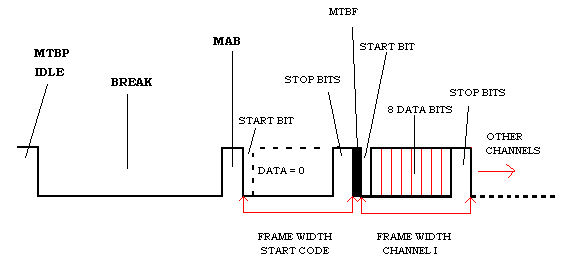
\includegraphics[width=15cm,scale=1]{resources/1_8-tramaDMX.png}
	\caption{Formato de la trama DMX. Fuente: \href{http://www.dmx512-online.com/packt.html}{LINK}}
	\label{fig:\thefigure}
\end{figure}

A cada trama con 512 canales se la llama "universo de DMX". Si se necesitan enviar más de 512 canales se utilizan más universos.

\subsubsection{Subcapa de control de acceso al medio}
DMX no implemente ningún mecanismo de control de acceso al medio debido a que el único transmisor es la red es el maestro y todos los esclavos reciben la misma información.

\section{Updown} \label{sec:\thesection}
\subsection{Definición}
El \textbf{Updown}, que se puede ver en la figura \ref{fig:1.9}, es básicamente una grúa que sube y baja una carga conforme a comandos recibidos por una equipo que utilice el protocolo DMX, como puede ser una consola de control de luminaria. La distancia máxima a la que la carga puede bajar es de 4 metros.

Este producto fue concebido en \textbf{Blackout}, una empresa productora y proveedora de tecnología cuyo objetivo es generar contenido audiovisual para grandes eventos. Blackout tomó interés en esculturas cinéticas como la de la figura \ref{fig:1.3} pero se encontró con el problema que el costo de importación de los equipos utilizados para tales fines, sumado a su precio unitario, era muy elevado. Por este motivo, decidió comenzar el desarrollo de un producto propio y nacional para alcanzar su objetivo.\\

\begin{figure}[!ht]
	\centering
	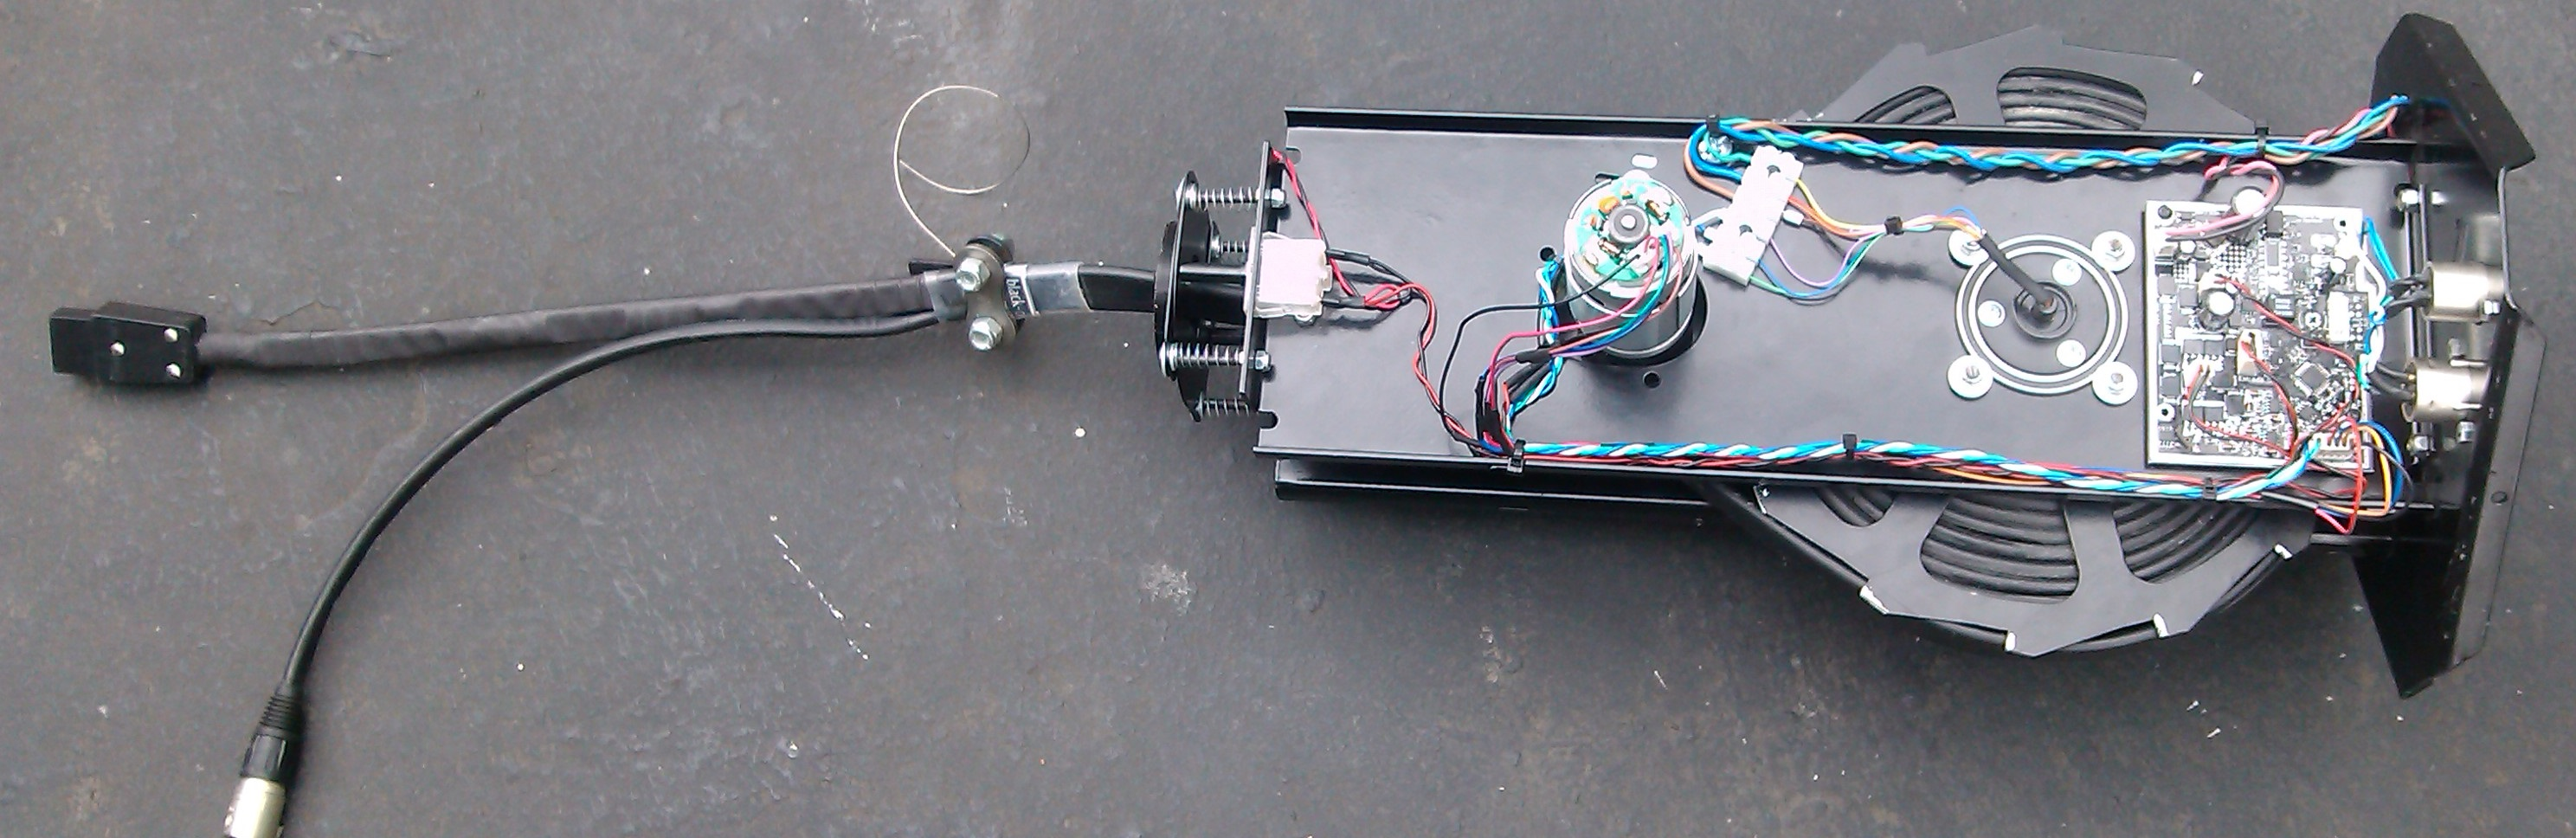
\includegraphics[width=15cm,scale=1]{resources/1_9-updown.jpg}
	\caption{Imágen del Updown, desarrollado por la empresa Blackout}
	\label{fig:\thefigure}
\end{figure}
\newpage
\subsection{Descripción del sistema}

En la figura \ref{fig:1.10} se presenta el diagrama general del equipo updown. Allí se pueden identificar todos elementos electrónicos y mecánicos que conforman el sistema, los agentes externos del sistema, y la comunicación entre ellos.

\begin{figure}[!ht]
	\centering
	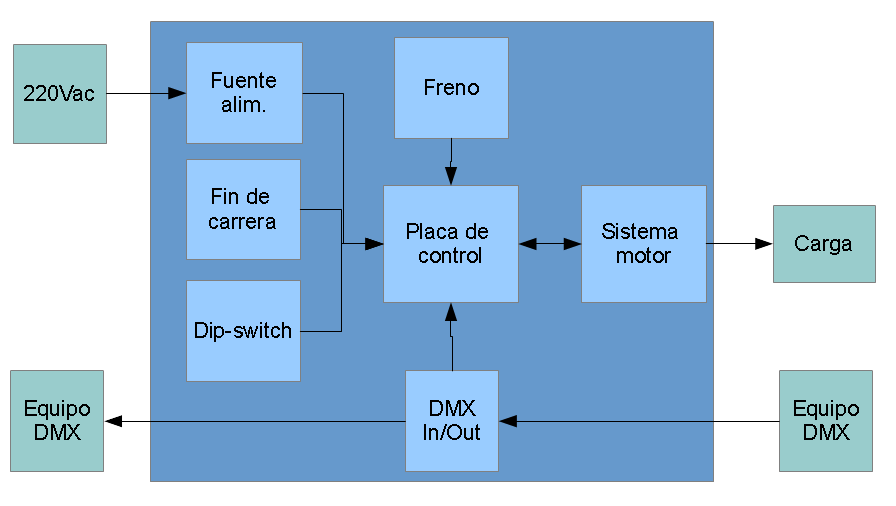
\includegraphics[width=15cm,scale=1]{resources/1_10-diagramaBasicoUpdown.png}
	\caption{Diagrama conceptual del equipo Updown}
	\label{fig:\thefigure}
\end{figure}

\subsubsection{Fuente de alimentación}
La fuente de alimentación es la encargada de proveer la potencia necesaria para el funcionamiento del sistema motor, y de placa de control junto con sus periféricos. Esto lo logra convirtiendo la tensión de red de 220Vac a una señal continua de 24Vcc, entregando 4.5A máximo.

\subsubsection{Entrada y salida DMX}
La señal DMX proveniente del master de la red, otro Updown, o cualquier otro equipo esclavo dentro del mismo universo DMX ingresa al sistema para ser procesada por la placa de control. Su función es indicarle al equipo la referencia de posición y velocidad, y los parámetros que correspondan a la carga.\\
Además, para cumplir con el estándar DMX, la señal de entrada se replica mediante un puente a una salida para que otro equipo pueda ser conectado a la red.

\subsubsection{Dip-switch}
El dipswitch consta con varios divisores resistivos, 10 switchs y un led indicador. Su función es seleccionar el canal inicial de DMX con el que el equipo trabajará.

\subsubsection{Freno}
El freno consta de una bobina, desactivada por defecto, que mueve una varilla metálica que traba el carrete que contiene la polea. Al activar la bobina la varilla libera al carrete, permitiendo el libre movimiento de la carga.

\subsubsection{Fin de carrera}
El fin de carrera consta de un par de pulsadores en la base del equipo. Eventos como enrollar completamente la polea activa alguno de los pulsadores, dandole aviso a la placa de control.

\subsubsection{Sistema motor}
El elemento principal del sistema motor es un motor de continua de 24V con un encoder AB en su eje. Este motor mueve un carrete en donde se enrolla el cable que sostiene la carga, que tiene un peso de 3Kg. El carrete, llamado disco, tiene unas marcas que son sensadas por un encoder en la placa de control para tener una segunda referencia de posición. La dirección de giro del motor se selecciona a través de un puente H.

\begin{figure}[!ht]
	\centering
	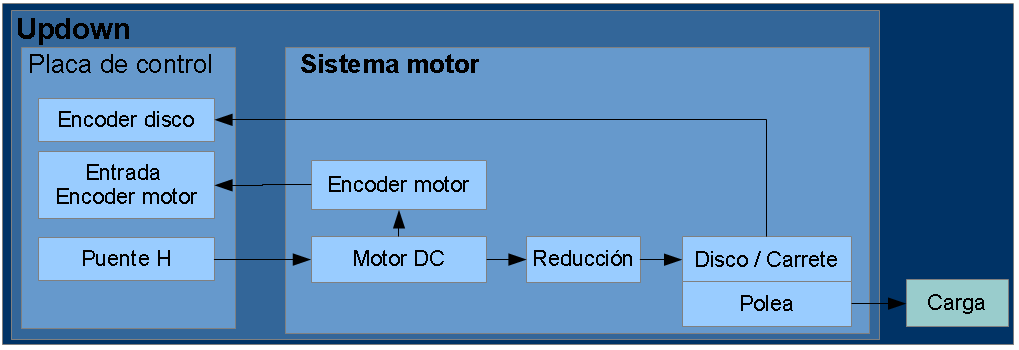
\includegraphics[width=15cm,scale=1]{resources/1_11-diagramaSistemaMotor.png}
	\caption{Diagrama del sistema motor}
	\label{fig:\thefigure}
\end{figure}

\subsubsection{Placa de control}
La placa de control contiene electrónica para el manejo de las entradas y salidas del sistema, y un controlador para manejar todos los periféricos siguiendo la lógica deseada.\\

\begin{figure}[!ht]
	\centering
	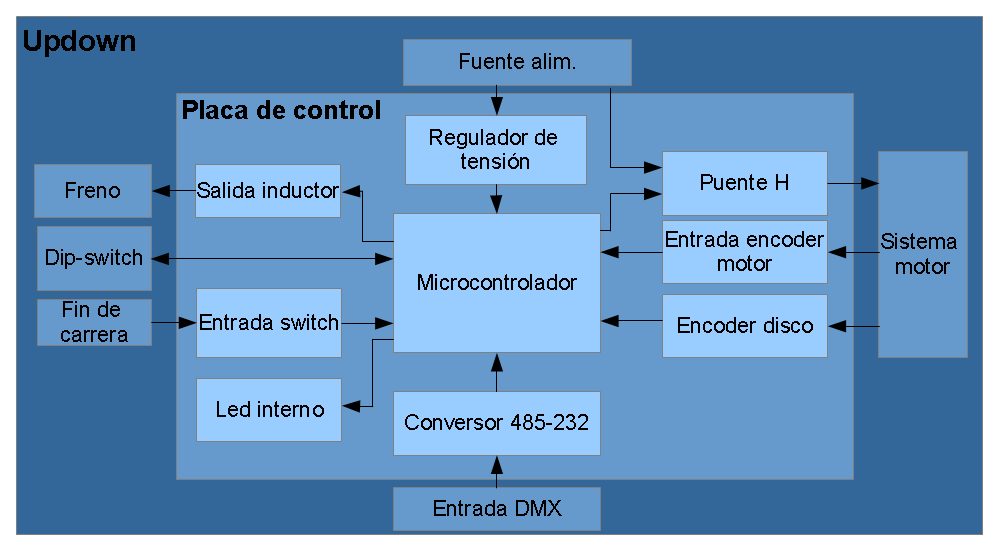
\includegraphics[width=15cm,scale=1]{resources/1_12-diagramaPlacaControl.png}
	\caption{Diagrama de la placa de control y su interacción con el hardware externo}
	\label{fig:\thefigure}
\end{figure}


\subsection{Resumen de entradas y salidas del sistema}
\subsubsection{Entradas} 
Señal de DMX, Fin de carrera, Dip-switch, Encoder AB de disco, Encoder AB de motor.\\
\subsubsection{Salidas}
Freno, Motor, Led interno (led indicador de la Placa de control), Led externo (led indicador del Dipswitch), Puente H.

\newpage
\section{Justificación del proyecto} \label{sec:\thesection}
Durante el desarrollo del updown la empresa se dió cuenta que con los recursos que contaban, tiempo en particular, no podían concretar los requerimientos que buscaban que el updown tuviera. 

Por este motivo, Blackout se vió en la necesidad de buscar a alguien externo a la empresa para darle fin al proyecto, lo que presentó la oportunidad de realizar el trabajo de concluir el desarrollo del equipo, que es en lo que este proyecto final se basa.

\section{Objetivos} \label{sec:\thesection}
El objetivo del proyecto es que el Updown suba y baje una carga de 3Kg, siguiendo las referencias de posición y velocidad dadas por un master DMX. Además, debe contar con ciertos mecanísmos de detección y manejo de errores para hacer que el producto sea seguro. También se tiene que terminar el desarrollo del dipswitch.\\
Como la mayoría del hardware del equipo resuelto las tareas a complir para terminar el producto, y dar por concluido el proyecto, se pueden resumur en los siguientes 4 requisitos:

\subsection{REQ-01}
Contar con el software necesario para el manejo de todas las entradas y salidas del sistema.
\subsection{REQ-02}
Lograr que las cargas manejadas por los equipos se muevan a la velocidad y posición indicadas mediante una consola DMX.
\subsection{REQ-03}
Manejar errores y excepciones de hardware para lograr que el producto sea seguro, siendo que será instalado en eventos con un alto nivel de concurrencia.\\
Dentro de estos errores se eneucntran: corte de cadena, pérdida de señal DMX y accionamiento indebido del fin de carrera.
\subsection{REQ-04}
Concluir el desarrollo del dipswitch.

%\subsection{Productos que compiten en el mercado}
%El equipos más conocido empleado para estas aplicaciones es el \href{http://www.eastsunlite.com/p31.html}{OrbisFly}, de \href{https://www.kinetic-lights.com/}{Kinetic Lights}. Estos dispositivos de orígen Chino trabajan con una esfera RGB de peso estándar de 1Kg, aunque soporta un peso máximo de 2Kg, que puede descender hasta 9 metros. Dispone de un display LCD y botoneras para el testeo y configuración el equipo\\






\chapter{Diseño}
\thispagestyle{empty}

\section{Descripción del capítulo} \label{sec:\thesection}
En este capítulo se analizan los requerimientos presentados en la sección \ref{sec:1.5} del capítulo 1 con el objetivo de describir la planificación para llevarlos a cabo.

\section{REQ-01} \label{sec:\thesection}
Para cumplir este requerimiento se debe contar con herramientas de software que permita el manejo de: freno, leds indicadores, fin de carrera, DIP-switch, encoders AB de disco y motor, motor y DMX. Además, como la placa de control no cuenta con un puerto de debug es necesario tener algún canal de comunicación alternativo, como un puerto serie por software. También será necesario temporizar ciertas partes del programa, por lo que se deberá poder manejar un timer.\\
El microcontrolador utilizado en la placa de control es el Atmega328p, y cuenta con periféricos para manejar todas las entradas y salidas del sistema por lo que es una buena elección para el proyecto. El único inconveniente que presenta es que es un microcontrolador de 8 bits con relativamente baja memoria y sin optimizaciones para operaciones de punto flotante. 

Para controlar el hardware del microcontrolador y sus periféricos internos y externos se necesitan bibliotecas, las cuales son un conjunto de funciones o procedimientos externos a la aplicación a desarrollar que le permiten al usuario manejar ciertos aspectos del sistema de forma más fácil.\\
Una opción es utilizar bibliotecas ya desarrolladas, entre las cuales se destacan las de Arduino. Arduino, una plataforma de programación de sistemas embebidos muy popular, utiliza en sus placas microcontroladores de marca Atmel. En particular, el \textit{Arduino UNO} utiliza el Atmega328p, por lo que existen funciones provistas por Arduino para el manejo de los periféricos del microcontrolador que se utiliza en el proyecto. \\
Otra opción es el desarrollo de bibliotecas a medida para el proyecto, desarrollando las funciones necesarias para el manejo de los periféricos que se necesiten para que se comporten exactamente como uno desea.\\
En la tabla \ref{table:2.1} se presenta una comparación entre ambas opciones.

El mayor problema con las bibliotecas de Arduino es que para que cuadren en proyectos grandes como estos requieren modificaciones, y las funciones provistas deben ser \\analizadas para verificar que no se usen elementos como delays bloqueantes ni operaciones de punto flotante indiscriminadamente, ya que deterioran el rendimiento. Además no está claro el uso de periféricos de hardware por parte de las mismas en su documentación factor que obliga a revisarla completamnete para descubrir las interdependencias entre partes de las mismas y qué sucede si se desea controlar directamente un cierto periférico. \\
Como el objetivo es hacer que el sistema sea lo más confiable posible, y teniendo en cuenta que el tiempo de desarrollo no es un factor crítico, \textbf{se desarrollarán bibliotecas propias en detalle para manejar los periféricos}.\\

\begin{table}[!ht]
	\begin{center}
		\begin{tabular}{|c|l|l|}
			\hline
			\rowcolor{OODlightblue}
			\textbf{} & \textbf{Arduino} & \textbf{Propia} \\
			\hline \hline
			Pros & - Listas para usar & - Bajo uso de recursos \\
			& - Altamente testeadas  & - Confiabilidad \\
			& - Mantenidas por una comunidad & - Predictibilidad \\
			\hline
			Cons & - Genéricas (poco optimizadas) & - Tiempo de desarrollo alto por defecto \\
			& - Necesitan modificaciones para ser útiles & - Investigación y estudio \\
			& - Requieren análisis &   \\
			\hline
		\end{tabular}
	\end{center}
	\caption{Comparación entre el uso de bibliotecas de Arduino vs el desarrollo de unas propias}
	\label{table:\thetable}
\end{table}

\section{REQ-02} \label{sec:\thesection}
\subsection{Esquema de control}
Para cumplir con este requerimiento la carga se debe mover en respuesta a una referencia de posición y a otra de velocidad indicadas por una consola DMX. Para esto se utilizará el esquema de control mostrado en la figura \ref{fig:2.1}, siendo: p la posición, v la velocidad,  Cp el controlador de posición, Cv el de velocidad, \(\varepsilon\)p y \(\varepsilon\)v los errores de posición y velocidad, u la acción de control, G la planta, y rp\_dmx y rv\_dmx las referencias de posición y velocidad dadas por la consola DMX.

\begin{figure}[!ht]
	\centering
	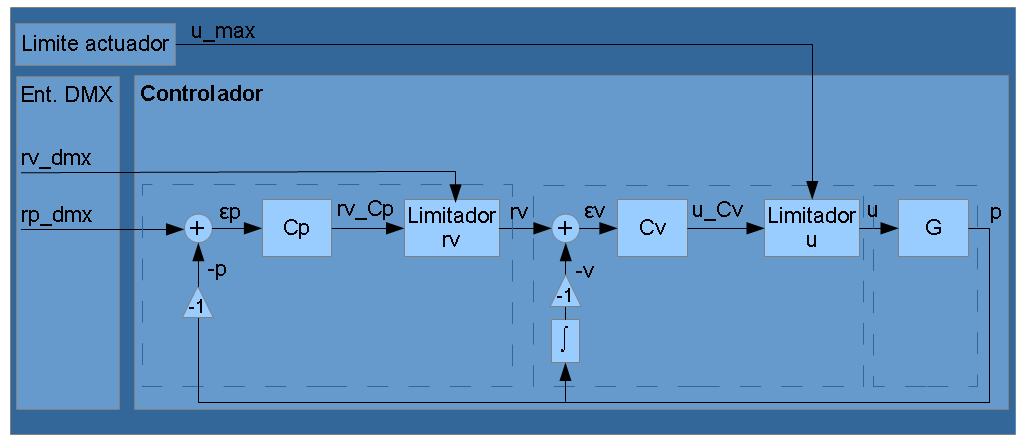
\includegraphics[width=16cm,scale=1]{resources/2_1-diagramaControlador.png}
	\caption{Esquema de control a implementar}
	\label{fig:\thefigure}
\end{figure}

La elección de este esquema fue debido a su simpleza: un controlador de velocidad se encarga de mantener la velocidad igual a la referencia, mientras que uno de posición le indica al de velocidad que debe frenar cuando la posición objetivo está por ser alcanzada. Para evitar que el controlador de posición le indique al de velocidad una referencia mayor a la permitida, se utiliza un limitador en al referencia de velocidad. Similarmente, como la acción de control será el ciclo de trabajo del pwm que mueve al motor, se utiliza un segundo limitador para evitar que el ciclo de trabajo supere el 100 \%.

La simpleza en el controlador y su modelo son un factor muy importante en este proyecto, ya que el objetivo es controlar el equipo mediante una consola DMX, y los efectos enviados por consola tienen una dinámica que el equipo debe seguir lo más fielmente posible. Introducir mucha dinámica por parte del controlador, por más que haga al sistema más estable, es indeseado en este caso. 

\subsection{Modelo de la planta}
Para este proyecto la planta será considerada como el conjunto motor-transmisión-carga. Un esquema mecánico de la planta se muestra en la figura \ref{fig:2.2}. Su funcionamiento es el siguiente: parte de la potencia eléctrica que ingresa al motor se transforma a mecánica y se utiliza para mover el piñón que se encuentra conectado al eje del motor. El piñon, a través de una cadena ANSI 25, transfiere su energía a la corona, que hace girar un disco adosado a ella. Este disco, o carrete, contiene en su interior el cable que sostiene a la carga, enrrollándolo o desenrrollándolo para subirla o bajarla. Como la carga del updown puede necesitar ser alimentada y recibir señal de DMX, el cable utilizado contiene en su interior 2 cables con ambas señales.

Ahora, para diseñar el controlador se debe encontrar un modelo matemático de la planta. Una opción es determinar las ecuaciones diferenciales que gobiernan el sistema aplicando la segunda ley de newton, y determinando el modelo matemático de un motor de continua mediante identificación. El problema es que por motivos constructivos del equipo existen muchas piezas que generan roces en diferentes partes del recorrido de la carga, lo que quiere decir que hay una perturbación cuya dinámica es totalmente desconocida y que depende de varios factores, como la distancia y el peso de la carga.\\
Por lo tanto, se abordará el problema con un método más simple: determinar el modelo de todo el conjunto mediante identificación, midiendo la respuesta del sistema ante ciertas entradas. Como el objetivo es que varios updown se comporten lo más parecido posible, se realizarán las pruebas para por lo menos 2 updown. 

\begin{figure}[!ht]
	\centering
	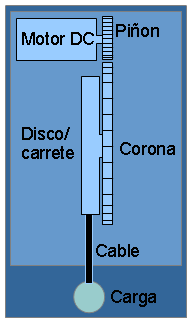
\includegraphics[width=6cm,scale=1]{resources/2_2-modeloMecPlanta.png}
	\caption{Modelo mecánico de la planta}
	\label{fig:\thefigure}
\end{figure}


\subsection{Procedimiento para el diseño de control}
Primero se determinará el período de muestreo y actuación inyectándole un escalón unitario a planta.\\
Luego, se obtendrá el modelo de la planta mediante identificación paramétrica, haciendo uso de un método de estimación de tipo offline (no recursivo) \cite{sec2_3_3}.\\
Paso seguido se diseñarán los controladores de posición y velocidad en base al modelo de la planta obtenido\\
Finalmente se validarán los controladores diseñados haciendo pruebas directamente sobre el equipo updown.

\subsection{Relación entre cuentas de encoder y distancia}
A medida que el motor gira desenrolla o enrrolla el cable para bajar o subir la carga respectivamente. Un problema de esto es que dependiendo cuán enrrollado está el cable en el disco un mismo número de cuentas de encoder se puede traducir en distintas distancias recorridas por la carga. Por ejemplo, si el cable está completamente enrollado cuando se gira 360 grados el carrete el largo desenrrollado será uno, mientras que si el cable se encuentra parcialmente desenrrollado la distancia descendida en un giro de 360 grados del carrete será menor que la anterior. Esto se debe a la variación del díametro debido a la acumulación del cable al estar enrrollado.\\
Para determinar esta relación se harán marcas sobre en el cable y para cada una se anotará el valor de cuentas del encoder del motor, que es el que más resolución tiene. Con estos datos se construirá una tabla, se encontrarán varios polinomios que ajusten los datos y se determinará cuál de ellos es el que se implementará en software.

\subsection{Velocidad máxima}
Una tarea a resolver es determinar cuál es la velocidad máxima posible para una carga determinada.

Para determinar este valor se medirá la velocidad para una carga de 3Kg en subida aplicando sobre el motor un PWM con ciclo de trabajo de 100\%.

La posición máxima posible queda dada por condiciones de diseño, siendo de 4 metros.

\section{REQ-03} \label{sec:\thesection}
En las siguientes secciones se detallan los errores que puede detectar el controlador del equipo.

\subsection{Corte de correa}
La transmisión de potencia entre el piñón en el eje del motor y la corona en el disco se hace a través de una correa. El problema es que durante las pruebas, la empresa observó que la correa podría cortarse. \\
La manera que tiene el equipo de detectar este error es mediante un segundo encoder AB que mide el giro del disco. Como la relación de vueltas entre el disco y el motor es proporcional, cualquier desviación grande de esta proporcionalidad indica que uno se está moviendo más rápido que el otro. Esto podría interpretarse como que la correa fue cortada o que alguno de los encoders dejó de funcionar, 2 errores válidos de hardware.

Para poder detectar estos errores lo primero que se hará es determinar la relación entre las cuentas del encoder del disco y las del motor. Luego verificará en el firmware que esta se cumpla en todo momento, bajo un cierto nivel de error aceptable. En caso de no cumplirse se accionará el freno, se detendrá el equipo completamente y se indicará sobre la existencia del error mediante el led de la placa de control (led interno).

\subsection{Fin de carrera}
La función principal del fin de carrera (un par de pulsadores en la base del equipo) es indicar cuándo el cable que sostiene la carga está completamente enrrollado para determinar la posición 0 o "home" del equipo, dado que este puede estar en cualquier posición al ser encendido.\\
La función secundaria del fin de carrera es detectar posibles eventos indeseados. Por ejemplo, en su punto más bajo la carga se encontrará a 4 metros por debajo del 0 del updown, por lo que podría comenzar a oscilar debido a fuertes vientos o personas que muevan la carga. Por cómo está construido el fin de carrera si la carga oscila más allá de un ángulo de aproximadamente 15 grados el fin de carrera se accionará dando aviso de esto.

Para poder detectar estos errores se verificará que el fin de carrera no sea presionado fuera de la rutina de calibración. En caso de que sea presionado en estas condiciones se detendrá el equipo, se esperará un tiempo a que la oscilación baje, e intentarán reanudar las operaciones normales. En caso de que el fin de carrera siga presionado se accionará el freno, se detendrá el equipo completamente y se indicará sobre la existencia del error mediante el led de la placa de control (led interno).


\subsection{Pérdida de señal de DMX}
El estándar DMX establece que el tiempo máximo entre un paquete de datos y otro, tiempo de IDLE o MTBP (ver tabla \ref{table:1.1}), es de 1 segundo. Esto quiere decir que si por 1 segundo no me llegaron nuevos datos se considera que se perdió la comunicación con el dispositivo DMX.

Para detectar la pérdida de señal de DMX se verificará constantemente que el último paquete haya llegado hace menos de 1 segundo. En caso de no cumplirse se asumirá que las referencias de posición y velocidad son 0 (equipo detenido en una posición segura). Además, por una convención en equipos DMX, se indicará mediante el led en el DIP-switch (led externo) cuándo el equipo recibe correctamente la señal de DMX y cuándo no, encendiéndolo y apagándolo rápidamente en el primer caso y lentamente en el segundo.


\section{REQ-04} \label{sec:\thesection}
El propósito del DIP-switch en el equipo es poder seleccionar el canal principal de DMX a partir del cual leer las referencias de posición y velocidad, dentro de los 512 canales que tiene un universo DMX. Para lograr esto cuenta con 10 switchs, 9 que determinan el canal de DMX (\( 2^9 = 512 \)) y uno extra para ampliaciones futuras. Estos conmutadores conectan o desconectan resistencias de unos divisores de tensión resistivos, variando el valor entregado por cada uno de ellos. Como el DIP-switch cuenta con 3 divisores se tienen 3 salidas analógicas, que dan información de qué switchs están activados y cuáles no. \\
El esquema de uno de los divisores se puede ver en la figura \ref{fig:2.3}. Para completar con el desarrollo del DIP-switch se deben encontrar 5 valores de resistencias (R1,R2,R3,R4 y R).

Para hallar estos 5 valores se simulará el divisor de tensión en Matlab, probando con distintas combinaciones de resistencias hasta que los valores analógicos de la salida para cada combinación de resistencia estén lo suficientemente separados.

\begin{figure}[!ht]
	\centering
	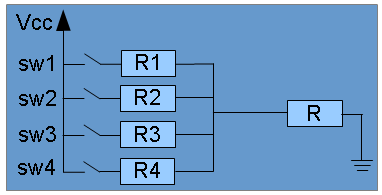
\includegraphics[width=12cm,scale=1]{resources/2_3-dipswitch.png}
	\caption{Diagrama de uno de los 3 divisores de tensión del DIP-switch}
	\label{fig:\thefigure}
\end{figure}

\newpage
\section{Firmware del updown} \label{sec:\thesection}
\subsection{Convenciones}
Con el objetivo de maximizar el encapsulamiento, las funciones dentro de los módulos se dividirán en privadas y públicas. Las privadas podrán ser accedidas únicamente por otras funciones dentro del módulo, mientras que las públicas también podrán ser accedidas por funciones de otros módulos. Para implementar esto se hará uso del concepto de "modularización por clases" \cite{sec2_6_2-1} en el cual se realiza la separación de información en archivos .c (código) y .h (headers). Los .h tendrán las declaraciones de funciones externas y definiciones para que, al ser incluido por otros módulos, tengan acceso a las mismas.\\
En cuanto a variables, solo se utilizarán variables internas al módulo. En caso de que tengan que poder ser accedidas externamente se implementarán setters (para escribir un valor en la variable) y getters (para obtener el valor de la variable) según corresponda.\\
Las funciones tendrán su nombre en formato \textit{camelCase} (primera letra minúscula y el resto de las primeras letras de las palabras utilizadas en el nombre en mayúscula), los macros (\#define) en \textit{MAYUSCULA}, y los módulos en formato PascalCase (como el camel case pero con la primera letra en mayúsucula).
Finalmente, todas las funciones y definiciones que pueden ser accedidas desde afuera de un módulo llevarán como prefijo el nombre del módulo seguido de un guión bajo. 

Además, debido a políticas de Blackout, todo el software desarrollado debe ser entendible por todo el equipo de trabajo. Esto quiere decir que una de las metas para las funciones de las bibliotecas a crear es que permitan un flujo entendible, y que los nombres de las funciones sean similares a las de Arduino ya que lo que se acostumbraba a utilizar en la empresa para la programación de sistemas embebidos.\\
Para lograr este objetivo todas los módulos desarrollados tendrán una función de inicialización llamada "init", y de lectura y escritura, según corresponda, llamadas "read" y "write", respectivamente. 

A contunuación se presentan algunos ejemplos de las convenciones que se usarán. Función de inicialización del módulo 1: Modulo1\_init(); Define del largo de un buffer genérico del módulo 3: Modulo3\_BUFFERGENERICO.


\subsection{Bibliotecas de bajo nivel}
Como se mencionó en la sección \ref{sec:2.2}, se desarrollarán bibliotecas para manejar los periféricos del Atmega328p y así poder controlar el hardware del sistema. Esto implica analizar la hoja de datos del Atmega328p \cite{sec2_6_2-2} e interactuar con los registros, un lugar de memoria utilizado para guardar información, que correspondan.\\ 
Asociadas a las bibliotecas viene de la mano el concepto de módulo, que tiene que ver con agrupar funciones similares en un mismo paquete para desacoplar dependencias y separar al sistema en varios subsistemas que sean lo más independientes que se pueda. Esto ayuda a que el programa sea escalable y mantenible, por lo que todo el software desarrollado se hará de manera modular.

Entonces, para manejar los periféricos se creará una biblioteca de bajo nivel que constará de los siguientes módulos:
\begin{itemize}
	\item \textbf{Entradas y salidas digitales}, para leer el estado del fin de carrera y comandar el freno, los leds indicadores interno y externo, y el puente H. Este módulo se llamará \textit{DigitalIO}.
	\item \textbf{Entradas analógicas}, para leer las 3 salidas analógicas del DIP-switch y poder determinar la posición de los selectores. Este módulo se llamará \textit{ADC}, por \textit{Analog to Digital Converter}.
	\item \textbf{Interrupciones externas} por cambio de estado de un pin, para llevar cuenta de los cambios de estado de los encoders AB y así saber la posición relativa. Este módulo se llamará \textit{EXINT}, por \textit{EXternal INTerrupts}.
	\item \textbf{PWM}, para el manejo del motor de continua. Este módulo se llamará \textit{PWM}, por \textit{Pulse Width Modulation}.
	\item \textbf{UART}, para la lectura de la señal DMX. Este módulo se llamará \textit{UART}, por \textit{Universal Asynchronous Receiver/Transmitter}
	\item \textbf{UART por software}, una UART implementada en pines genéricos que se utilizará para el depuración de la placa. Este módulo se llamará \textit{SUART}, por \textit{Software UART}.
	\item \textbf{Base de tiempo}, un timer utilizado para la temporización tareas y eventos. Este módulo se llamará \textit{Tick}.
\end{itemize}

\subsection{Bibliotecas de alto nivel}
Si bien la biblioteca de bajo nivel permite acceder a las entradas y salidas del equipo, se necesita otra biblioteca, de alto nivel, que utilice sus módulos para manejar el hardware como se espera. Por ejemplo, no es lo mismo obtener un valor analógico leyendo un \textit{registro} (lugar para el almacenamiento de datos) del microcontrolador, que determinar qué conmutadores del DIP-switch están activados leyendo 3 valores analógicos, aunque ambas acciones involucren leer una entrada analógica.\\
Entonces, se creará una biblioteca más acorde a la aplicación y no tan genérica como la de bajo nivel, que constará de los siguientes módulos:
\begin{itemize}
	\item \textbf{DIP-switch}, que incluye la lectura de las llaves del DIP-switch, y la escritura del led indicador externo.
	\item \textbf{Grua}, que incluye el manejo del motor, del led interno, del freno y del fin de carrera.
	\item \textbf{DMX}, para la recepción de datos de la consola DMX.
	\item \textbf{Encoder}, para el manejo de los encoders AB del disco y del motor.
	\item \textbf{Controlador}, para la implementación del sistema de control
\end{itemize}

\subsection{Arquitectura en capas de los módulos de firmware}
De estas 2 bibliotecas se obtiene el diagrama en capas presentado en la figura \ref{fig:2.4}, el cual muestra su relación, dependencia y alcance. Por encima de ellas se encuentra la capa de aplicación, que hará uso de estas bibliotecas, relacionándolas con el objetivo de que el Updown funcione como debe.

\begin{figure}[!ht]
	\centering
	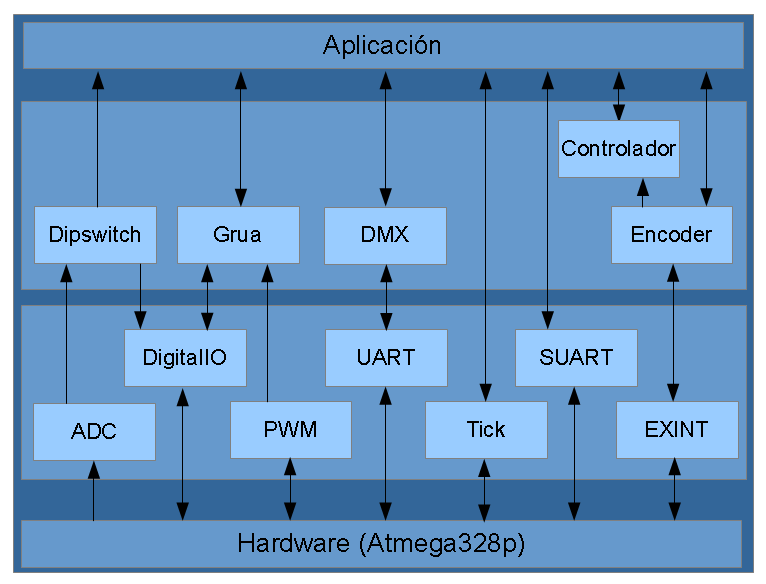
\includegraphics[width=14cm,scale=1]{resources/2_4-diagramaDeModulos.png}
	\caption{Diagrama de módulos del firmware}
	\label{fig:\thefigure}
\end{figure}

\chapter{Desarrollo}
\thispagestyle{empty}

\section{Descripción del capítulo} \label{sec:\thesection}
En este capitulo se desarrollarán las soluciones propuestas en el capítulo de diseño. Esto implica detallar el proceso realizado, describir los cambios que se debieron hacer en caso de que el planteo inicial no haya funcionado, análisis de resultados, etc.

\section{Firmware del updown} \label{sec:\thesection}

\subsection{Librerías de bajo nivel}
Todas las librerías de bajo nivel fueron desarrolladas en base a la hoja de datos del Atmega328p.

\subsubsection{DigitalIO}
El desarrollo del módulo de entradas y salidas digitales (DigitalIO) está basado en el capítulo 18 de la hoja de datos del Atmega328p.
\subsubsection{ADC}
El desarrollo del módulo ADC está basado en el capítulo 28 de la hoja de datos del Atmega328p.

\subsubsection{PWM}
El desarrollo del módulo PWM está basado en el capítulo 20 de la hoja de datos del Atmega328p.

\subsubsection{EXINT}
El desarrollo del módulo de interrupciones externas (EXINT) está basado en el capítulo 17 y 18 de la hoja de datos del Atmega328p.

\subsubsection{UART}
El desarrollo del módulo UART está basado en el capítulo 24 de la hoja de datos del Atmega328p.

\subsubsection{SUART}
El desarrollo del módulo SUART está basado en el capítulo 19 de la hoja de datos del Atmega328p.

\subsubsection{Tick}
El desarrollo del módulo Tick está basado en el capítulo 22 de la hoja de datos del Atmega328p.

\subsection{Librerías de alto nivel}

\subsection{Funcion principal}

\section{Controlador} \label{sec:\thesection}

\subsection{Relación entre cuentas de encoder y distancia}
Como se mencionó en la sección \ref{sec:2.3}, subsección 3, 

\subsection{Determinación de la velocidad máxima}

\subsection{Obtención del período de muestreo}
Como se mencionó en la sección \ref{sec:2.3}, subsección 3, 

\subsection{Obtención del modelo de la planta}

\subsection{Obtención del controlador}

\subsection{Ajuste del controlador}


\section{Dipswitch} \label{sec:\thesection}



\chapter{Validación}
\thispagestyle{empty}

\section{Análisis} \label{sec:\thesection}
En este capítulo se mostrarán los ensayos realizados para validar los requerimientos presentados en la sección \ref{sec:1.5}. Esto incluye:
\begin{itemize}
	\item \textbf{REQ-01:} validar que firmware desarrollado para el equipo maneja correctamente todas las entradas y salidas.
	\item \textbf{REQ-02:} validar que la carga sigue la posición y velocidad indicada por DMX .
	\item \textbf{REQ-03:} validar que el comportamiento del sistema ante el descubrimiento de uno de los 3 errores detectables es la esperada. 
	\item \textbf{REQ-04:} verificar que el funcionamiento del dipswitch es correcto.
\end{itemize}

\section{Validación del requerimiento REQ-03} \label{sec:\thesection}
Para validar el requerimiento REQ-03 se realizaron 3 pruebas.
\subsection{Pérdida de DMX}
Si el equipo recibe señal de DMX el led externo debe cambiar de estado a razón de 4 veces por segundo, y mantener el estado si se perdió la señal por más de un segundo.

Para verificar que esto se realizaron las siguientes pruebas:
\begin{enumerate}
	\item Se conectó el equipo a la red, sin el cable de DMX conectado. El led externo se mantiene apagado.
	\item Se conecto el cable DMX con la consola prendida. El led externo comienza a parpadear a una frecuencia de 2Hz.
	\item Se desconecta el cable DMX de la consola. El led externo deja de parpadear transcurrido 1 segundo de haber desconectado el cable.
\end{enumerate}
Con esto se verifica que el comportamiento es el deseado.	
	 
\subsection{Accionamiento indebido del fin de carrera}
Idealmente, el fin de carrera solo debe accionarse una vez durante la rutina de calibración para determinar el 0 de posición. En caso de que se accione fuera de este escenario la carga debe frenar por 6 segundos, y volver a subir al 0 de posición. En caso que el FDC esté presionado por más de 15 segundos se debe parar el motor, poner el freno, y el led interno debe cambiar de estado cada 2 segundos.

Para verificar que esto se realizaron las siguientes pruebas:
\begin{enumerate}
	\item Luego de que la etapa de calibración concluye, se le indica al equipo que baje la carga 2 metros (velocidad al 50\%). Durante el descenso se acciona el fin de carrera una vez y se espera. Al accionarlo, la carga para durante 6 segundos, y comienza a subir lentamente al 0 de posición. Luego intenta bajar nuevamente y llega a la posición deseada.
	\item Partiendo de una posición de 2 metros, se le indica al equipo que suba la carga 1 metro (velocidad al 50\%). Durante el ascenso se acciona el fin de carrera una vez y se espera. Al accionarlo, la carga para durante 6 segundos, y comienza a subir lentamente al 0 de posición. Luego intenta subir nuevamente y llega a la posición deseada.
	\item Partiendo de una posición de 1 metro, se mantiene presionado el fin de carrera. Durante este tiempo la carga baja lenta y continuamente hasta que pasan 15 segundos. En ese momento la carga para, se activa el freno, y el led interno titila a una frecuencia de 0.25Hz.
\end{enumerate}

El comportamiento en la tercer prueba es el esperado ya que como se mantiene el fin de carrera presionado automáticamente "se llega al 0", y en consiguiente la carga baja 10 cm, como es de esperarse. Luego se pasa al modo normal, pero como el fin de carrera sigue presionado se vuelve a entrar al de calibración, y el ciclo vuelve a comenzar denuevo, repitiendose hasta que transcurren 15 segundos.

Por lo tanto, con esto se verifica que el comportamiento es el deseado.
	
\subsection{Corte de cadena}
Si la relación entre el encoder de disco y de motor se desvía mucho de la dada por la tabla \ref{table:3.2} el se debe detener el motor y accionar el freno para evitar que la carga baje. Además, el led interno debe cambiar de estado 2 veces por segundo.

Para verificar que esto se realizaron las siguientes pruebas:
\begin{enumerate}
	\item Se desconecta el cable que asocia el encoder del motor y la placa de controlcausando que las cuentas del encoder de motor dejen de cambiar. Luego de un segundo el motor para y el freno se acciona, deteniendo completamente la carga. Adicionalmente, el led interno titila a una frecuencia de 1Hz.
	\item Se desconecta el cable que asocia el encoder del disco y la placa de control  causando que las cuentas del encoder de disco dejen de cambiar. Luego de un segundo el motor para y el freno se acciona, deteniendo completamente la carga. Adicionalmente, el led interno titila a una frecuencia de 1Hz.
\end{enumerate}
Para verificar completamente que el comportamiento ante un error es el deseado se debería, además de probar la pérdida de cuenta de los encoders, probar cortando la cadena. Como no se logró hacer esto con el equipo en funcionamiento este punto no se pudo validar totalmente. Sin embargo, es muy poco probable que se corte la cadena debido a la dureza de la misma y a que la carga es de solamente 3 Kg.

\section{Validación de los requerimientos REQ-01, 02 y 04} \label{sec:\thesection}
Los requerimientos REQ-01, REQ-02 y REQ-04 se validan simplemente controlando al updown mediante DMX. De esta manera se verifica funcionamiento de todos ellos ya que se utilizan todas las entradas y salidas (asociado a la validación del REQ-01), el sistema de control (asociado a la validación del REQ-02) y el dipswitch (asociado a la validación del REQ-04).

La prueba se realiza con 4 equipos updown dispuestos en forma de matriz de 2x2, como se muestra en la figura \ref{fig:4.1}, colgados a 4 metros sobre el nivel del piso. Todos tienen en su extremo una carga de 3Kg, que es una luminaria cuyas intensidades R, G y B pueden ser controladas mediante 3 canales de DMX.

\begin{figure}[!ht]
	\centering
	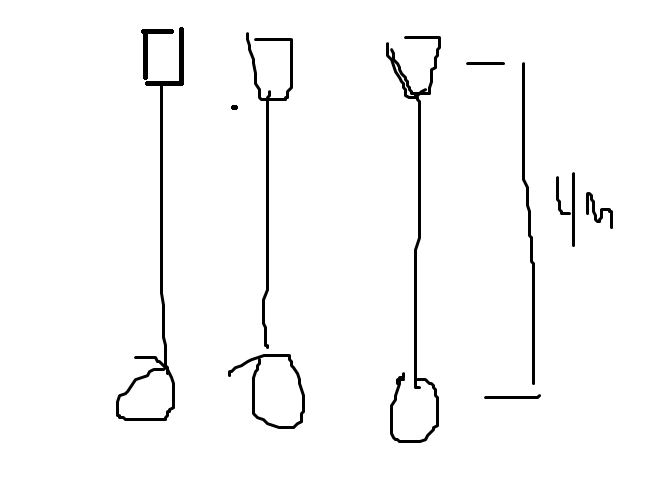
\includegraphics[width=10cm,scale=1]{resources/4_1-disposicionUpdowns.png}
	\caption{Disposición de los equipos Updown, vista frontal}
	\label{fig:\thefigure}
\end{figure}

Para manejar los equipos se utiliza la consola \href{http://www.lighttrader.com/images/HI61020007_L.JPG}{HedgeHog 4}, de HighEnd Systems. En ella se programan 2 rutinas:
\begin{itemize}
	\item \textbf{Rutina 1}: los 4 equipos se mueven juntos, a velocidad máxima, a las posiciones 0, 1, 2, 3 y 4 metros, en subida y en bajada.
	\item \textbf{Rutina 2}: los 4 equipos se mueven a posiciones distintas (apelando al direccionamiento por dip switch) y la velocidad varía con el tiempo.
\end{itemize}

\subsection{Direccionamiento de los equipos}
Cada updown recibe 2 canales DMX, uno de posición y otro de velocidad, mientras que las cargas, que se configuran independientemente, reciben 3 canales (R, G y B). Además, en las instalaciones de equipos DMX por convención los equipos se direccionan de atras para adelante, de izquierda a derecha.

Esto quiere decir que, refiriendose a la figura \ref{fig:4.1}, el updown A tendrá la dirección 1, el B la dirección 3, el C la 5 y el D la 7. Para lograr esto se configuran los dipswitch como corresponde. Por ejemplo, el dipswitch del equipo C tendrá la llave 2 y 3 activadas, lo cual se traduce a address 5 en el programa.\\
Por otro lado, las cargas (L en la figura) se las configura en la dirección 10. Esto se hace manualmente desde un display digital que las luminarias traen. 

En la figura \ref{fig:4.2} se muestra cómo se vizualizan los canales en la consola HOG, y a qué estará asociado cada uno. 

\begin{figure}[!ht]
	\centering
	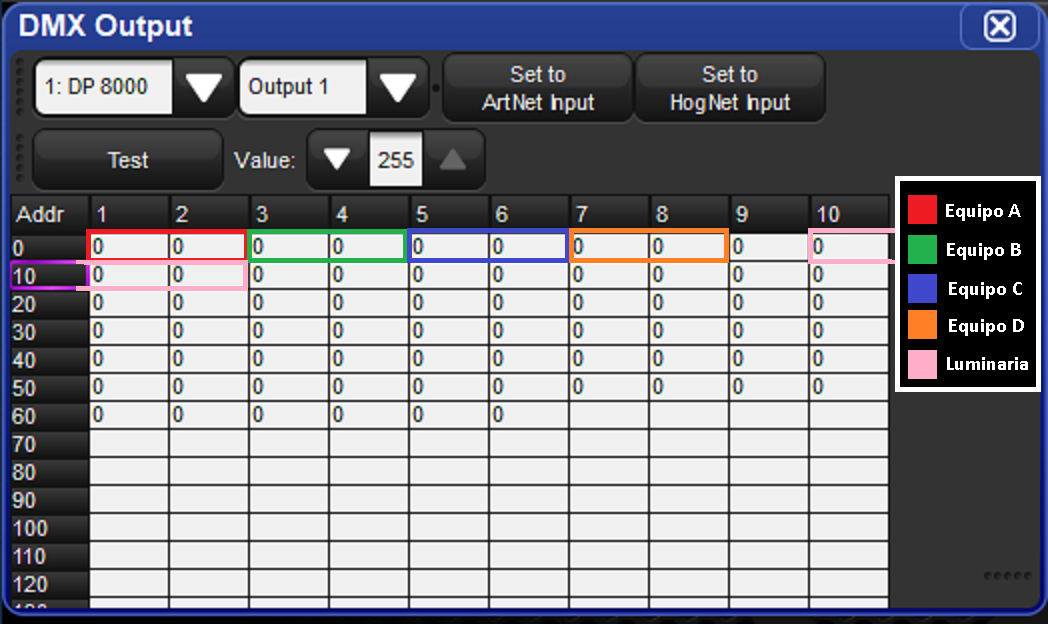
\includegraphics[width=15cm,scale=1]{resources/4_2-direccionamiento.png}
	\caption{Canales DMX asociados a los updown y las cargas}
	\label{fig:\thefigure}
\end{figure}

\subsection{Rutina 1}
Se programa en la consola rutina mostrada en la figura \ref{fig:4.3}, en donde los equipos cambian de posición constantemente, en ascenso y descenso, de 0 a 4 metros. \\
Adicionalmente se cambian los colores de la luminaria del equipo C a medida que esta se mueve. La secuencia es: rojo para 0 metros, verde para 1 metro, azul para 2 metros, amarillo para 3 metros y blanco para 4 metros.\\
Para permitir que las posiciones sean alcanzadas antes de pasar a la siguiente se le agrega a cada instrucción un delay de 7 segundos, motivo por el cual las 8 instrucciones llevan el texto "Follow + 7s". El follow simplemente significa que luego de terminada la instrucción en curso y transcurridos los 7 segundos, se ejecuta automáticamente la próxima.
	
\begin{figure}[!ht]
	\centering
	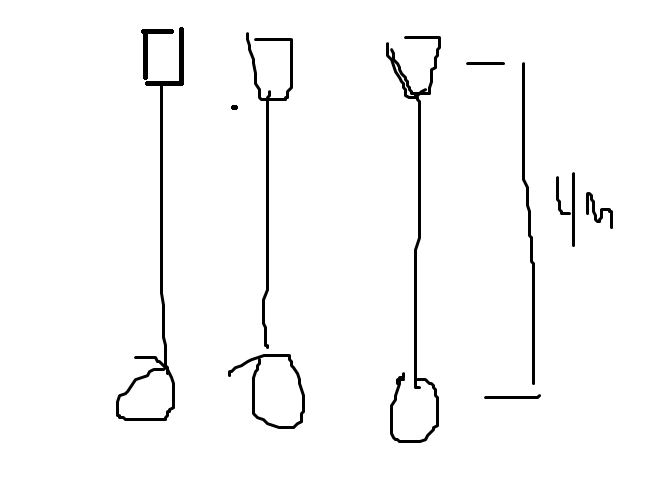
\includegraphics[width=12cm,scale=1]{resources/4_3-cuelist1.png}
	\caption{Rutina 1, programada en la consola}
	\label{fig:\thefigure}
\end{figure}

Las posiciones obtenidas de la prueba se pueden ver en la figura \ref{fig:4.4}. Para cada una se midió el error de posición cuando las cargas llegan al objetivo para verificar la presición del equipo. De estas mediciones se obtuvo que los errores de los equipos se encuentran siempre dentro de las \( \pm 120 \) cuentas. De la tabla \ref{table:3.2} se ve que 25cm son 1130 cuentas del encoder del motor, por lo que 120 cuentas son aproximadamente 2.5cm.\\
Si bien estos son los resultados de error para los 4 equipos, se puede ver en la figura \ref{fig:4.4} que el error del equipo D (el del frente a la derecha). Si bien no se nota claramente en la imágen, el cable del equipo se encuentra bastante torcido aproximadamente 2.5 metros por encima de la carga, lo cual puede, entre otras cosas, ser el causante de esta diferencia de posición, error que la placa de control no contempla.

\begin{figure}[!ht]
	\centering
	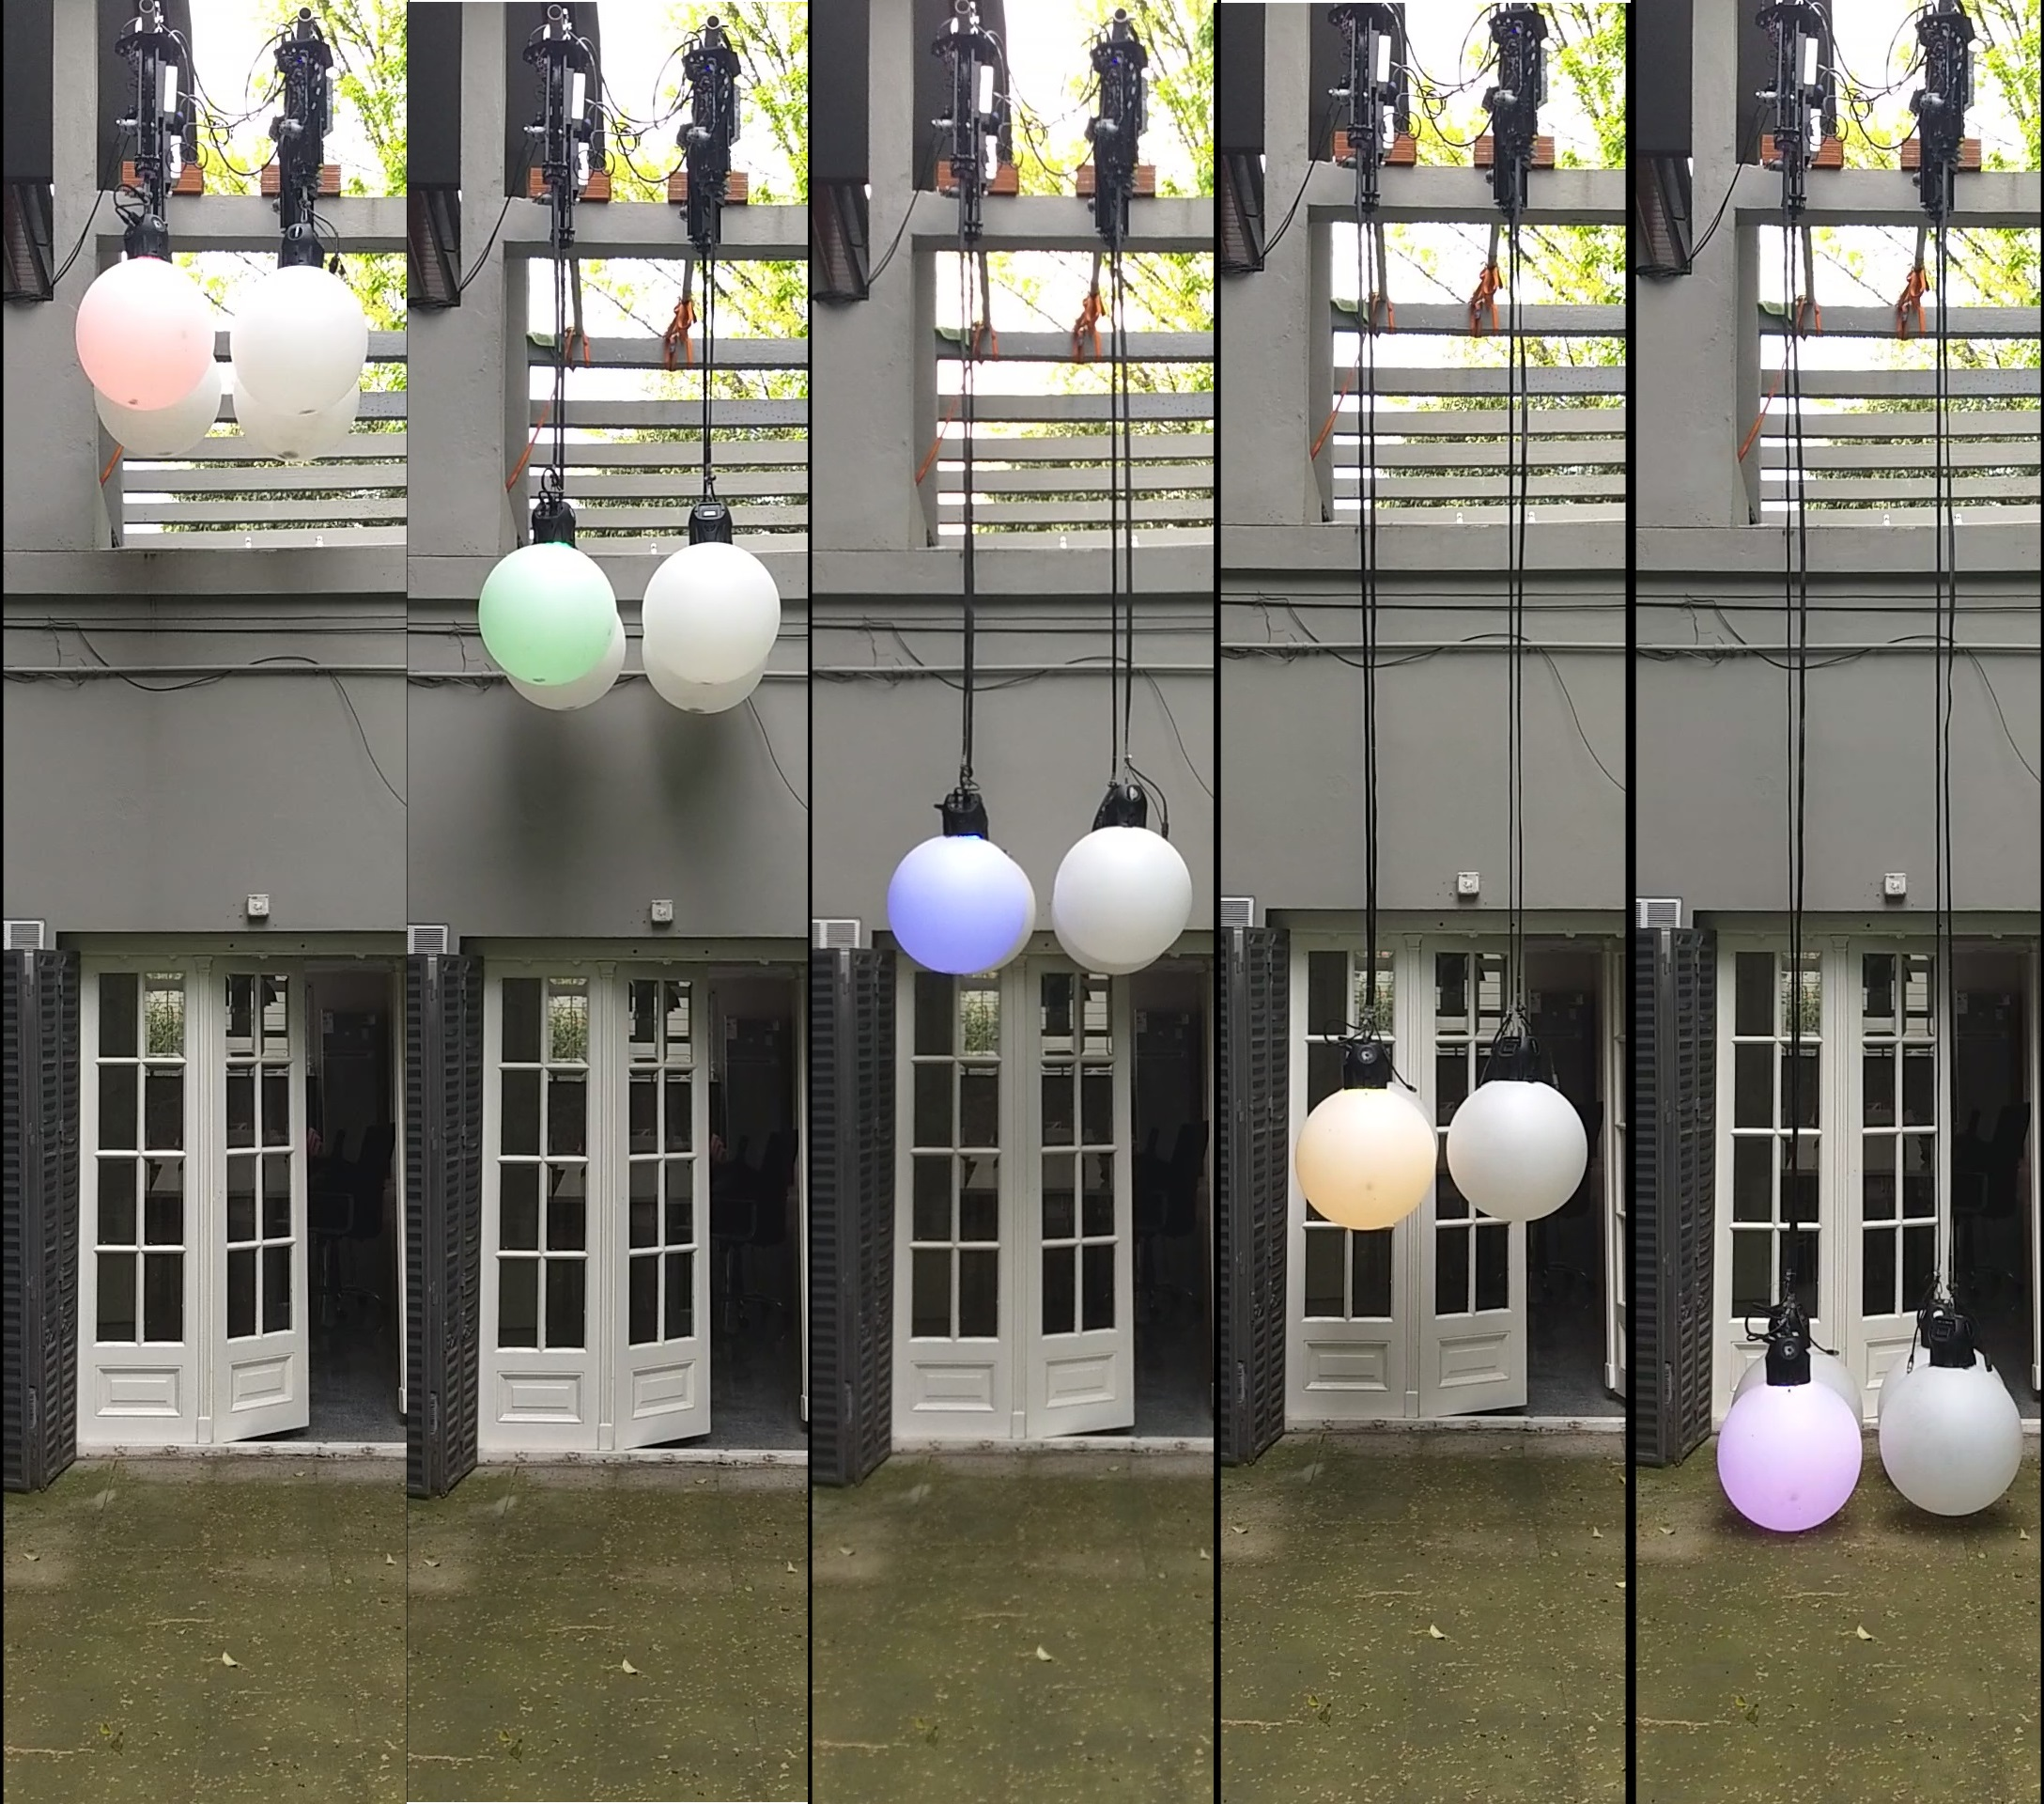
\includegraphics[width=16cm,scale=1]{resources/4_4-cuelist1_resultados.jpg}
	\caption{Muestra de posiciones para la rutina 1}
	\label{fig:\thefigure}
\end{figure}

En la figura \ref{fig:4.5} se muestra cómo quedan los canales para, por ejemplo, la instrucción "Pos 3m, Vel 100\%" (las instrucciones número 2 y 8 de la figura \ref{fig:4.3}). Los valores 192 en los canales DMX 1, 3, 5 y 7 corresponden a la posición de las cargas, que es 3 metros siendo 255 4 metros, mientras que los valores 255 en los canales 2, 4, 6 y 8 corresponden a la velocidad del 100\%. Por otro lado, los canales 10 y 11, los cuales contienen las intensidades R y G de las luminarias, tienen un valor de 255, por lo que la intensidad en esos 2 colores es máxima (notese que se distinguen los colores de la luminaria a pleno día).

\begin{figure}[!ht]
	\centering
	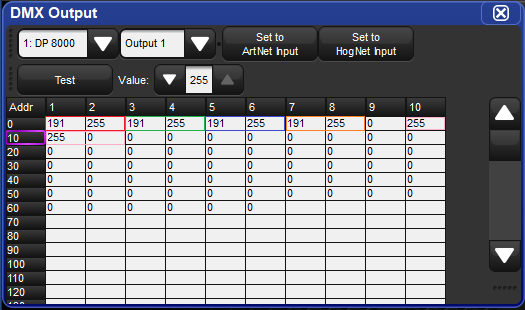
\includegraphics[width=16cm,scale=1]{resources/4_5-cuelist1_cue2.png}
	\caption{Valores de los canales para la instrucción "Pos 3m, Vel 100\%"}
	\label{fig:\thefigure}
\end{figure}

Para constatar que la velocidad de los equipos es la correcta se midió la de los 4 equipos durante la prueba. Tanto para el ascenso como para el descenso la velocidad en régimen permanente de los 4 equipos es de \(40 \pm 1\) cuentas cada 20 milisegundos, lo cual concuerda con lo encontrado en la sección \ref{sec:3.3}, subsección 2, en donde se halló que la velocidad máxima posible es de 2 cuentas por milisegundo.

\subsection{Rutina 2}
En este caso se programa en la consola la secuencia mostrada en la tabla \ref{table:4.1}, en donde las cargas cambian de posicion y velocidad con cada nueva instrucción. En la figura \ref{fig:4.6} se muestran algunas de las posiciones alcanzadas durante esta prueba. \\
Al igual que en la rutina 1 el tiempo que se tarda de pasar de una instrucción a otra es de 7 segundos, por lo que en este caso las posiciones finales no llegan a ser alcanzadas para velocidades distintas a 100\% (el caso de la instrucción 1).

\begin{table}[!ht]
	\begin{center}
		\begin{tabular}{|c|c|c|c|c|c|c|}
			\hline
			\rowcolor{OODlightblue}
			Equipo & Pos. 1 & Vel. 1 & Pos. 2 & Vel. 2 & Pos. 3 & Vel. 3\\
			
			A & 1 m & 100\% & 2 m &  25\% & 3 m &  50\% \\
			
			B & 2 m &  & 1 m &  & 2 m &   \\
			
			C & 2 m &  & 3 m &  & 2 m &   \\
			
			D & 3 m &  & 2 m &  & 1 m &   \\
			\hline
		\end{tabular}
	\end{center}
	\caption{Rutina 2. Cada par posición,velocidad representa una instrucción}
	\label{table:\thetable}
\end{table}

\begin{figure}[!ht]
	\centering
	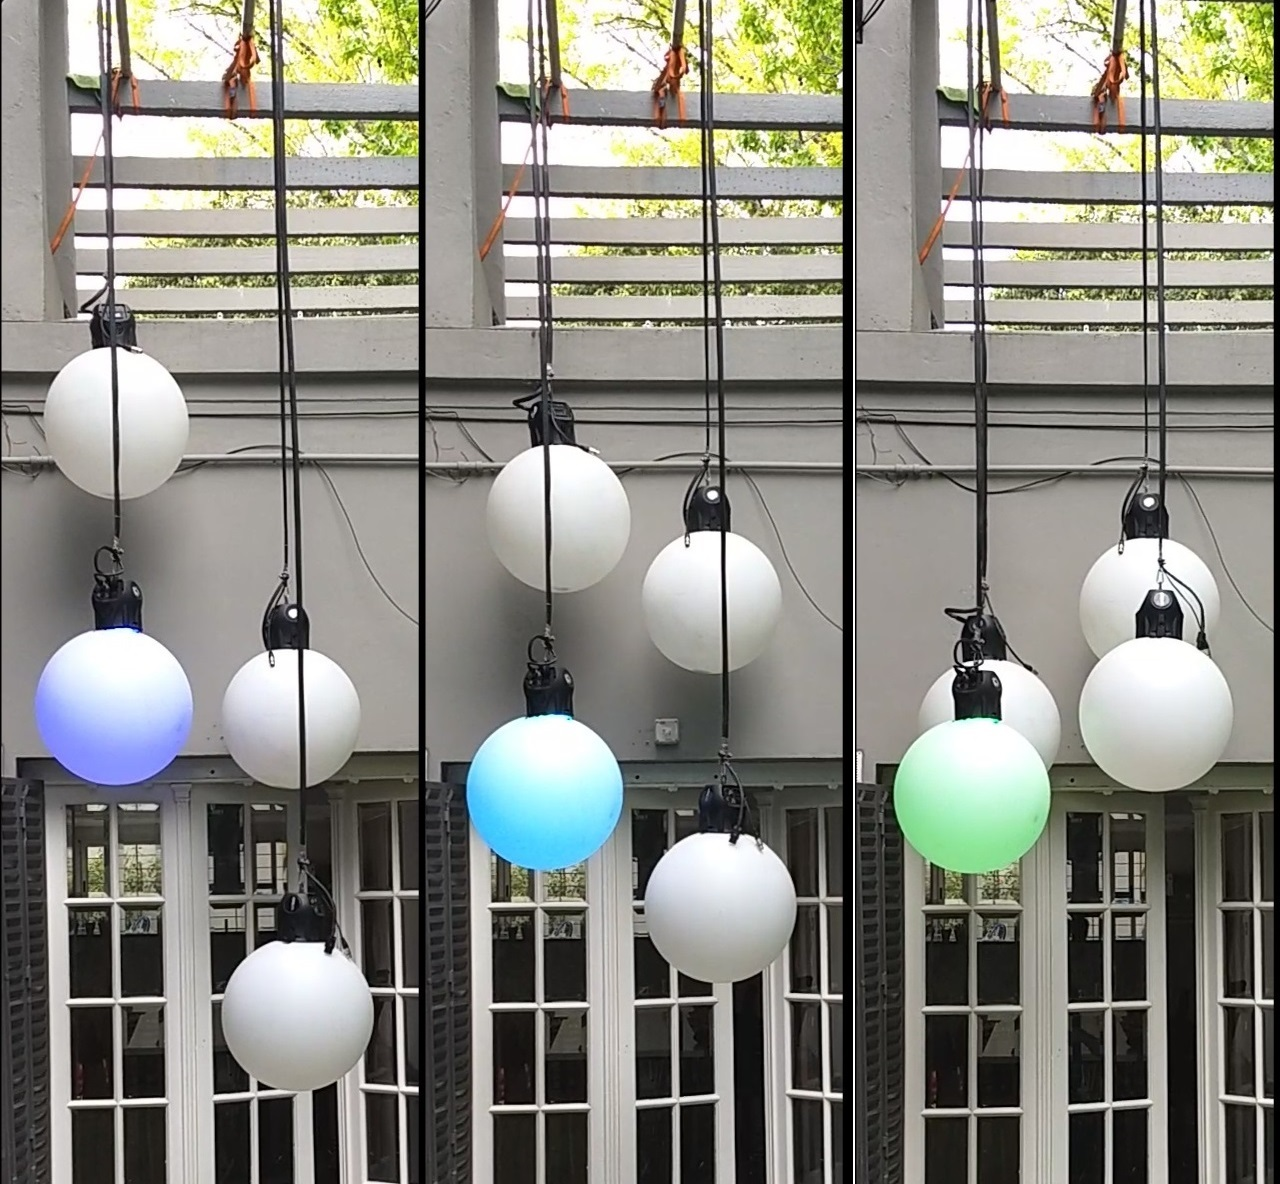
\includegraphics[width=14cm,scale=1]{resources/4_6-cuelist2_resultados.jpg}
	\caption{Muestra de posiciones para la rutina 2}
	\label{fig:\thefigure}
\end{figure}

Nuevamente se constataron las velocidades de los 4 equipos para cada instrucción. Para la instrucción 1 (velocidad de 100\%) la velocidad obtenida es de \(40 \pm 1\) muestras cada 20 ms, para la 3 (velocidad de 50\%) es de \(20\) muestras cada 20 ms y para la 2 (velocidad de 25\%) es de 10 muestras cada 20 ms, lo cual concuerda con lo esperado.







\chapter{Conclusiones}
\thispagestyle{empty}

\section{Conclusiones}

\section{Mejoras a futuro}

\section{Referencias utilizadas}

\end{document}